\documentclass[11pt,english,german]{report}

% Package import, Document Settings
\usepackage[a4paper,inner=3.5cm,outer=2.5cm]{geometry}
\usepackage[english,ngerman]{babel}
\usepackage[utf8]{inputenc}

% Packages
\usepackage{caption}
\usepackage{latexsym}
\usepackage[T1]{fontenc}
\usepackage{graphicx}
\usepackage{hyperref}
\usepackage{tabularx}
\usepackage{etoolbox}
\usepackage{fancyhdr}
\usepackage{amsthm}
\usepackage{mathtools}
\usepackage[xindy]{glossaries}
\usepackage{hyperref}
\usepackage{lastpage}
\usepackage{float}
\usepackage{makecell}
\usepackage{ltablex}
\keepXColumns
\usepackage{csquotes}

\newcommand{\pb}[1]{\parbox[t][][t]{1.0\linewidth}{#1} \vspace{-2pt}}

% clear default
\fancyhead{}
\fancyfoot{}

\pagestyle{fancy}
\fancyhf{}
\renewcommand{\headrulewidth}{0pt} % optional
\fancyfoot[L]{Kapitel: \nouppercase{\leftmark}}
\fancyfoot[R]{\thepage/\pageref{LastPage}}

% Redefine the plain page style, Chpater page
\fancypagestyle{plain}{%
  \fancyhf{}
  \renewcommand{\headrulewidth}{0pt} % optional
  \fancyfoot[R]{\thepage/\pageref{LastPage}}
}

\renewcommand{\chaptermark}[1]{\markboth{\MakeUppercase{#1}}{}}

% Glossar
\newglossaryentry{ATAS}
{
    name={ATAS},
    description={Aplinist Tracking \& Alerting System}
}
\newglossaryentry{entry}
{
	name={TTN},
	description={The Things Network, LoraWan Netzwerk}
}

\newglossaryentry{Blockierung}{name={Blockierung},description={Als Blockierung werden alle Notfälle bezeichnet, bei denen BerggängerInnen infolge Erschöpfung, Überforderung,
		Materialverlust oder anderen Missgeschicken nicht mehr in der Lage sind, ihre Tour aus eigener Kraft weiterzuführen
		oder abzubrechen. In der Regel sind die Betroffenen unverletzt.}}

\theoremstyle{definition}
\newtheorem{exmp}{Beispiel}[subsection]

\newglossaryentry{bergnotfall}{name={bergnotfall},description={Der Begriff „Bergnotfall“ umfasst alle Vorkommnisse, bei denen BerggängerInnen die Hilfe der Bergrettungsdienste beanspruchen. Dies betrifft auch Erkrankungen und Evakuationen von unverletzten Personen}}
	
\makeglossaries

\setcounter{secnumdepth}{2}
\setcounter{tocdepth}{1}

\begin{document}
\pagestyle{empty} %Keine Kopf-/Fusszeilen auf den ersten Seiten.
\begin{titlepage}
\begin{center}

% Oberer Teil der Titelseite:

\includegraphics[width=0.08\textwidth]{img/bfh_logo.png}\\[1cm]    
\textsc{\LARGE Bern University of Applied Sciences}\\[1.5cm]
\textsc{\Large Bachelor Thesis}\\[0.2cm]
\textsc{\Large Studiengang Informatik}\\[0.5cm]

% Title
\newcommand{\HRule}{\rule{\linewidth}{0.3mm}}
\HRule \\[0.4cm]
{\huge Alpinist Tracking \& Alerting System}\\[0.3cm]
{\huge \bfseries  ATAS}
\HRule \\[2cm]


\includegraphics[width=0.2\textwidth]{img/atas_logo.png}\\[2.5cm]    

% Author und Lehrer
\begin{minipage}{0.3\textwidth}
\begin{flushleft} \large
\emph{Autor:}\\
Martin \textsc{Schmidli}\\
\end{flushleft}
\end{minipage}
\hfill
\begin{minipage}{0.3\textwidth}
\begin{flushleft} \large
\emph{Betreuer:} \\
Mohamed \textsc{Mokdad}
\end{flushleft}
\end{minipage}
\hfill
\begin{minipage}{0.38\textwidth}
\begin{flushleft} \large
\emph{Experte:}\\
Daniel \textsc{Voisard}, BAKOM\\
\end{flushleft}
\end{minipage}

\vspace{20mm}

% Unterer Teil der Seite
Bern, {\large \today}
\end{center}
\end{titlepage}
\pagestyle{fancy}


\tableofcontents

% Mgmt Summary
% GLOSSAR, 3


%- Portieren der Software auf ES32, DONE
%- TTN als Platform, DONE, 
% SPI Schnittstelle analyse, was schickt die Lorwan library
%- Bitrate + laufzeit Analyse
%- Minimierung 


% Management Summary, 1

% Testdaten, Vorbereitung SFP7-SFP12, 2

% Testing erweitern was soll getestet werden 1
% Testszenarien, Wanderungen dokumentieren 1

% LoraWan Airtime, 1
% LoraWan ADR, 3
% Prototyp Display, 3
% Technologien, Alternative, Warum LORA? 2

% OK OK OK 
% Atas-Node2, Antenna Design, Short 3
% Motivation, 3, OK
% Einleitung Projekt 2, 1 OK
% Projekt einleitung detailiert, 1 OK
% Bilder Atas-Node2, 2 OK
% Bilder einzelner Atas-Node2 Module, 2 OK
%  Aufbau Gateway Doku, 1



\chapter*{Management Summary}
% 
Viele Bereiche des öffentlichen Lebens wurden durch eine digitale Revolution umgekrempelt. Waschmaschinen werden Smart, Roboter putzen das Haus, Autos fahren selbstständig. Das Thema IoT und Mobile Computing sind allgegenwärtig. Was aber passiert in der Bergwelt? Im Jahr 2016 kam es zu über 2800 Unfälle in den Schweizer Alpen. Viele Personen wurden verletzt, 178 endeten gar tödlich \cite{sacaccident}. Was werden dort für Fortschritte gemacht um das Risiko zu minimieren? Wie schreitet dort die Digitalisierung vorwärts? Nur selten spricht jemand von diesem Bereich. Der Fokus der großen Konzerne liegt wohl eher auf den angesprochenen Bereichen, dort wo es viel Geld zu holen gibt, dem Massenmarkt. Wäre es aber nicht auch wichtig in die Sicherheit in den Bergen zu investieren? Wie viele Unfälle könnten verhindert, wie viele Leben gerettet werden?\\[0.3cm]
Genau hier setzt das ATAS Projekt an. ATAS ist ein von mir erdachtes System welches auf der Basis von IoT Technologien versucht die Wahrscheinlichkeit für einen Unfall in den Bergen zu verkleinern. Das während dem Bachelor Thesis Vorprojekt (Projekt 2) erstellte Konzept, bildet die Grundlage für diese Thesis.\\[0.3cm] Der Bericht gliedert sich in 4 Bereiche. Im ersten Teil der Thesis wird die Funktionalität und der Aufbau des Systems genauer erläutert. Der Bericht startet mit einem groben System-beschrieb und wird später immer detaillierter. Im Vordergrund stehen hier die  Aufgabe der einzelnen Komponenten (Hard und Software) und deren Kommunikation untereinander. Im zweiten Teil geht es um die Technologien welche das System verwendet. Warum wurde diese gewählt und wie werden diese eingesetzt. Im dritten Teil wird der Aufbau eines neuen Hardware Prototypen beschrieben. Der im Vorprojekte aufgebaute Prototyp weißt einige Schwachstellen auf und muss verbessert werden. Im vierten Schritt wird das ATAS System getestet. Im Fokus liegen hier die Neuerungen beim Prototypen sowie die Datenübertragung zwischen den Komponenten. Am Ende werde ich ein Fazit aus den Tests ziehen und bewerten, ob dieses System einen praktischen Nutzen bietet und Alltagstauglich ist.

\chapter*{Motivation}
21.01.2017. Region Zweisimmen. Es war ein schöner Tag für eine Schneeschuhwanderung. Meine Kollegin und ich machten uns bereit. Wir schlüpften in die Schneeschuhe, packten die Skistöcke und zogen los. Meter für Meter kämpften wir uns den Weg zum Gipfel vor. Nach 3 Stunden hartem und schweißtreibenden Aufstieg gelangten wir schlussendlich zum Bergkamm. Die Aussicht war unser Lohn.
\begin{figure}[H]
	\centering
	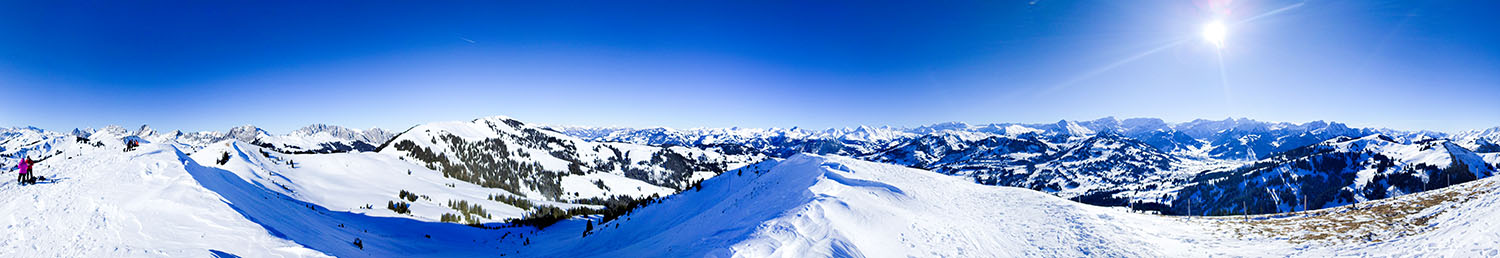
\includegraphics[width=\textwidth]{img/alps_panorama.jpg}
	\caption[Motvation Alpen Panorama]
	{Motivation Alpen Panorama}
\end{figure}
\noindent
Ich bin kein extrem Bergsteiger. Ich genieße die Schweizer Alpen, bin aber nie in hohen(3000m+) und gefährlichen Regionen unterwegs. Die Schneebedingungen wärend meiner Touren sind meist ideal. Die Gefahr ist minimal. Nur selten werden Themen wie Lawinen und daraus resultierendes Unfallverhalten in der Gruppe diskutiert.\\[0.3cm]
An eben diesem Tag stellten wir uns die Frage: Was wäre wenn?. Was wäre passiert wenn wir von einer Lawine verschüttet worden wären? Wer hätte uns gesucht, hätte uns überhaupt jemand gesucht. Falls meine Kollegin verschüttet wäre, wie lange würde es dauern bis die Rettungskräfte eintreffen würden? Wäre das Handynetz verfügbar gewesen? Und so weiter...\\[0.3cm]\
Diese Thematik beschäftigte mich noch lange. Als es schließlich darum ging ein Thema für das Bachelor Thesis Vorprojekt (Projekt 2) auszusuchen, wollte ich mich weiter mit diesen Fragen auseinandersetzen. Dank meinem Studium und der gewählten Fachrichtung 'Mobile Computing' hatte ich bereits ein, zwei Idee wie man diese Problematik angehen könnte. Das Projekt ATAS war geboren. Meine Vorstellung war es ein System zu erstellen, welches Personen in solchen Situation unterstützen, mehr noch solche Situationen verhindern sollte.\\[0.3cm]

\chapter*{Danksagung}
TODO
PRIO 3


\chapter{Einleitung}
Ein Gipfel gehört dir erst, wenn du wieder unten bist - denn vorher gehörst du ihm.\\[0.3cm]
\textbf{Hans lander, Italienischer Bergsteiger\cite{kammerlander}} \\[0.5cm]
\noindent
Die Berge sind eine faszinierende Landschaft. Viele Menschen gehen wandern, Ski fahren oder gehen Eisklettern. Die Anzahl der möglichen Aktivitäten ist schier grenzenlos. Immer wieder kommt es in dieser Idylle aber zu schweren Unfällen. Ausgelöst durch Steinschläge, Lawinen, Abstürze der Bergsteigenden/Alpinisten und vielen weiteren möglichen Ursachen. Der Schweizer Alpenclub (SAC) führt dazu eine Statistik \cite{sacaccident}. Nachfolgend ein kleiner Auszug aus der Bergunfallstatistik 2016. Die Grafik zeigt eine Übersicht der Anzahl Situationen wo eine Rettungsdienst ausrücken musste. Zu den Rettungsdiensten gehört beispielsweise die REGA.\\
\begin{figure}[H]
	\centering
	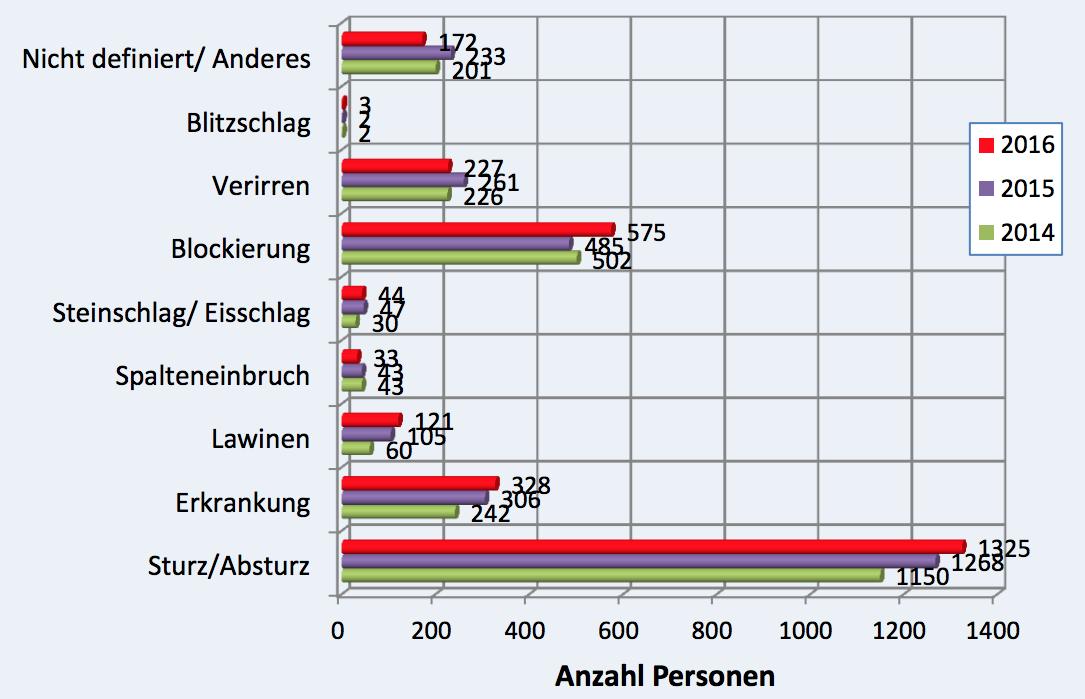
\includegraphics[width=\textwidth]{img/sac_accidentstatistic_2016_reason.png}
	\caption[Bergunfallstatistik 2016 - Notfallsituationen nach Unrsachen]
	{Bergunfallstatistik 2016 - Notfallsituationen nach Ursachen}
\end{figure}
\noindent
Die Vorfälle sind nach Ursache gegliedert. Zusammengefasst ergeben sich 2828 Notsituationen, wovon 178 tödlich endeten.

\newpage
\section{Projektidee}
Stellen Sie sich ein kleines mobiles Gerät vor, nachfolgend Tracker genannt, welches Skifahrern, Wanderer usw. abgegeben werden kann. Das Gerät sendet die Position der Person an einen Empfänger, nachfolgend Gateway genannt. Der Gateway wird bei der Talstation oder im nächsten Bergdorf montiert. Der Gateway sendet die empfangenen Daten der Tracker an eine zentrale Stelle irgendwo im Internet. Die Administratoren des Systems, beispielsweise die Rega, können schlussendlich über eine Webseite die aktuelle Position der Personen in den Bergen mitverfolgen und überwachen.

\section{Vorarbeiten}
Das Projekt 2 ist eine Projektarbeit welche im Laufe des Informatikstudiums absolviert werden muss. Diese Arbeit habe ich im vorhergehenden Semester (Frühlingssemester 2017) durchgeführt. Ziel dieses Projektes, war es das in der Einleitung beschriebene System technisch umzusetzen.\\[0.3cm]
Diese Bachelor Thesis baut auf den Erkenntnissen und Resultaten aus dem Projekt 2 auf.

\section{Aufgabenstellung}
Ziel der Bachelorarbeit soll es sein, dass während dem Projekt2 aufgebaute System intensiv zu testen und zu verbessern. Die Arbeit umfasst die folgenden Aufgaben.
\begin{itemize}
\item
Der Tracker soll in realer Umgebung getestet werden bspw. während einer Wanderung. Die Messdaten werden erfasst und analyisert.
\item Der Tracker Prototyp soll verbessert werden. Die dazu erforderlichen Massnahmen werden während der Bachelorarbeit spezifiziert und umgesetzt. Am Ende der Arbeit soll eine klare Aussage gemacht werden können ob das erdachte System praxistauglich ist
\item
Die während dieser Arbeit geleisteten Arbeiten sollen in einem Bericht dokumentiert werden.
\end{itemize}

\section{Rahmenbedingungen}
Die Rahmenbedingungen dieses Projektes wurden gemeinsam mit dem Betreuer definiert
\begin{itemize}
\item Die Bachelorarbeit baut auf der Arbeits des Projekt 2 auf. Die erstellete Hard und Software wird weiterverwendet.
\item The Things Network dient als Plattform für die Kommunikation unter den Komponenten.
\item Als Programmiersprache soll C/C++ verwendet werden
\item Auf den Einsatz eines Betriebsystememes auf dem Tracker Node soll verzichtet werden
\end{itemize}

\section{Technologien}
Sie als Leser denken nun vielleicht: "Das ist überflüssig. Ich habe doch mein Handy für so etwas? Schreib doch eine App!". Diese Aussage mag auf die touristischen Wander- und Skigebiete zutreffen. Der Empfang ist meistens wunderbar. Verlasssen wir diese 'sicheren' Orte und bewegen uns aber in höheren Lagen, wird der Empfang mit dem Handy immer schlechter oder existiert gar nicht. \bigskip \\
Aus diesem Grund mussten für dieses Projekt andere Technologien gefunden werden. In diesem Projekt werden folgende Technologien eingesetzt:
MQTT, LoRa, LoRaWAN\bigskip \\
Die verwendeten Technologien und der Grund für deren Einsatz werden in einem späteren Abschnitt genauer erklärt.

\section{Anwendungsfälle}
Dieses Abschnitt soll Ihnen erläutern, wie das ATAS System genutzt werden kann.
\begin{itemize}
	\item 
	Wenn in den Bergen eine Lawine ausgelöst wird, kann deren Position mit den Positionen der Tracker verglichen werden. Befindet sich ein Tracker in der Gefahrenzone, kann die Rettungsmannschaft sofort reagieren und ausrücken. Dieser Prozess läuft sofort ab und kann dabei die Überlebenschance der Opfer erhöhen. 
	\item 
	Wurden Personen von der Lawine begraben und der Tracker hat überlebt, könnte das Gerät weiterhin die Position senden. Kombiniert mit modernen Lawinensuchgeräten können die Einsatzkräfte gezielter nach Überlebenden suchen. Wenn keine Übertragung mehr möglich ist, wissen die Überwacher zumindest den letzten Aufenthaltsort. Das ATAS System hat nicht das Ziel Lawinensuchgeräte zu ersetzen, es ist eher als Ergänzung zu verstehen. 
	\item 
	Bewegt sich Tracker auf eine Gefahrenzone zu, beispielsweise ein Gebiet mit erhöhter Steinschlaggefahr, könnte die Person frühzeitig davor gewarnt werden. 
	\item 
	Ist es zu einem Unfall gekommen, kann der Alpinist mittels Tracker ein Notsignal absetzen. Dazu muss der Benutzer nur auf den Notfallknopf drücken.
\end{itemize}

\chapter{Systembeschreibung - Grob}
Um die nachfolgenden Kapitel zu verstehen, ist es sehr wichtig, sich mit der im Projekt 2 erstellten Systemarchitektur und die Terminologie vertraut zu machen. Die Architektur wurde im Vergleich zum Projekt 2 um einige Komponenten ergänzt.

\section{Grobe Systemarchitektur}
Dieser Abschnitt bietet Ihnen einen groben Überblick über die Benutzer, die Komponeneten und deren Beziehung innerhalb des ATAS Systems. Alle Einheiten werden auf den nachfolgenden Seite detailliert beschrieben.

\newpage
\section{Aufbau}
\subsection{Diagram}
Grobes Schema des ATAS Systems. Auf der nachfolgenden Seiten sind die einzelnen Komponenten im Detail beschrieben.\\[0.3cm]
\begin{figure}[H]
	\centering
	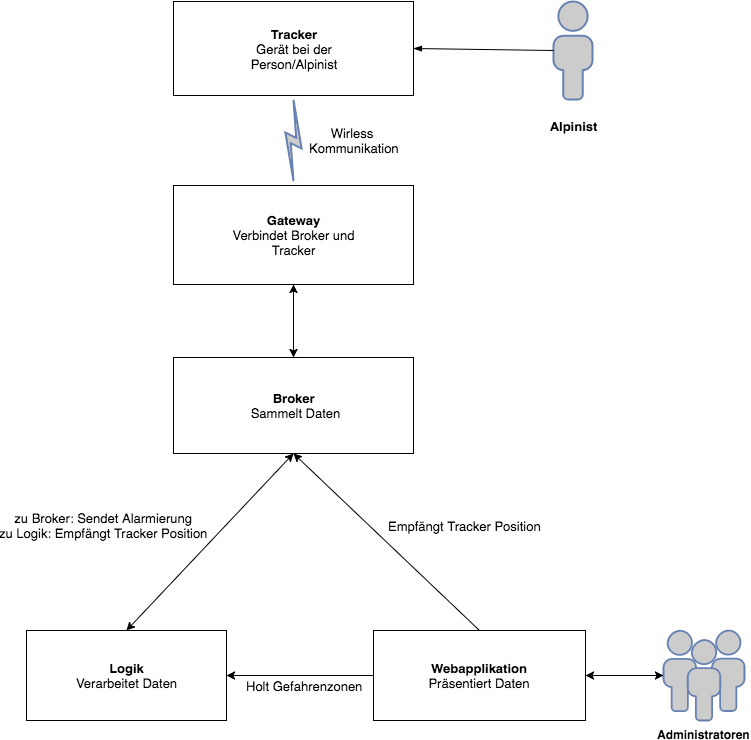
\includegraphics[width=\textwidth]{img/system/ATAS_SystemOverview_Abstract_BA.png}
	\caption[Atas Schema Grob]
	{Atas Schema Grob}
\end{figure}

\newpage

\subsection{Benutzer}
Die nachfolgenden Gruppen wurden als Benutzer des Systems identifiziert.
\subsubsection{Aplinist}
Alpinist wird als Generalisierung für Personen, welche sich in den Bergen aufhalten verwendet. Dazu gehören bspw. Wanderer, Skifahrer, Bergbauern usw.
\subsubsection{Überwacher}
Rettungsdienste wie bspw. die Rega oder die AirGlacier. Spitäler oder die lokalen Tourismusbehörden.

\subsection{Komponenten}
Das ATAS System besteht aus den nachfolgenden Komponenten. Komponenten sind als Hardware und Software zu verstehen.
\subsubsection{Tracker}
Stellen Sie sich ein kleines mobiles Gerät vor, nachfolgend genannt Tracker. Der Alpinist trägt den Tracker bei sich bspw. in einem Rucksack.\bigskip \\ 
Der Tracker verfügt über ein Display, Taste, GPS Modul, Kommunikationsmodul (Lora) und ein Lautsprecher.
\begin{itemize}
\item
Taste: Mit dem Druck auf den Knopf können die Überwacher über eine Notsituation aufmerksam gemacht werden. Bspw. Wenn der Alpinist einen Unfall hatte und nun bewegungsunfähig ist.
\item
Lautsprecher: Über den Lautsprecher kann der Alpinist über eine Gefahrenquelle mit einem akustischen Signal aufmerksam gemacht werden. Bspw. Wenn sich der Alpinist in einem Bereich am Berg mit erhöhter Gefahr für Lawinen aufhält. Der Lautsprecher dient zur Information, \textbf{dass ein Problem besteht}.
\item
Display: Über ein Display können mehr Informationen zum Tracker und den Gefahrenzonen angezeigt werden. Das Display dient zur Information, \textbf{was für ein Problem besteht}.
\item
GPS Modul: Der Tracker verfügt über ein GPS Modul. Mit dem GPS Modul kann die Position des Tracker auf der Erde ermittelt werden.
\item 
Lora Modul: Mittels Lora Modul können Daten an einen Empfänger, nachfolgend \textbf{Atas-Gateway} genannt, gesendet werden.
\end{itemize}

\subsubsection{Gateway}
Ein Gerät welches mit den Trackern bidirektional kommuniziert. Der Gateway wird an einem Ort nahe den Bergen installiert. Als mögliche Orte kommt ein Dorf im Tal oder eine Talstation in Frage.\bigskip \\
Der Gateway senden die empfangenen Daten an eine zentrale Datenmanager, nachfolgend \textbf{Broker} genannt.

\subsubsection{Broker}
Sammelt und speichert Daten. Der Broker kommuniziert mit den Gateways. Zusätzlich bietet der Broker ein Interface zum Abfragen und senden von Daten.

\subsubsection{Webapplikation}
Die Notfalldienste resp. Überwacher nutzen eine Webapp zum interagieren mit dem ATAS System. Die Webseite bietet folgende Funktionalitäten
\begin{itemize}
	\item
		Zeigt die Position der Tracker auf einer Karte an 
	\item
		Mittels der Webapp können Gefahrenzonen hinterlegt werden.
	\item 
		Zeigt an ob sich ein Tracker in einer Gefahrenzone aufhält.	
\end{itemize}

\subsubsection{Business Logik}
Die BusinessLogik umfasst Software welche berechnet, ob sich ein Tracker in einer Gefahrenzone aufhält. Wenn sich der Tracker in einer Gefahrenzone aufhält, senden das System eine Alarm an den Tracker. Das Signal gelangt via Broker und dem Gateway zum Tracker.

\newpage
\chapter{Systembeschreibung - Detail}
Die vorhergegangene grobe Architekturbeschreibung gibt einen guten ersten Überblick über das System. Technische Details zu  den verwendeten Technologien oder den genauen Fluss der Kommunikation ist nicht ersichtlich. In diesem Abschnitt soll nun intensiv auf diese Thematik eingegangen werden.\\[0.3cm]
Auf der nachfolgenden Seite finden Sie ein Schema welches einen genauen Überblick über das System liefert.\\[0.3cm]
Die Komponenten werden in 2 Kategorien eingeteilt. Komponenten mit einem blauen Kästchen wurden im Rahmen dieser Arbeit selbständig programmiert. Gelbe Kästchen markieren einen bestehenden Service welcher für den Aufbau des Systems implementiert wurde. 

\newpage
\begin{figure}[H]
	\centering
	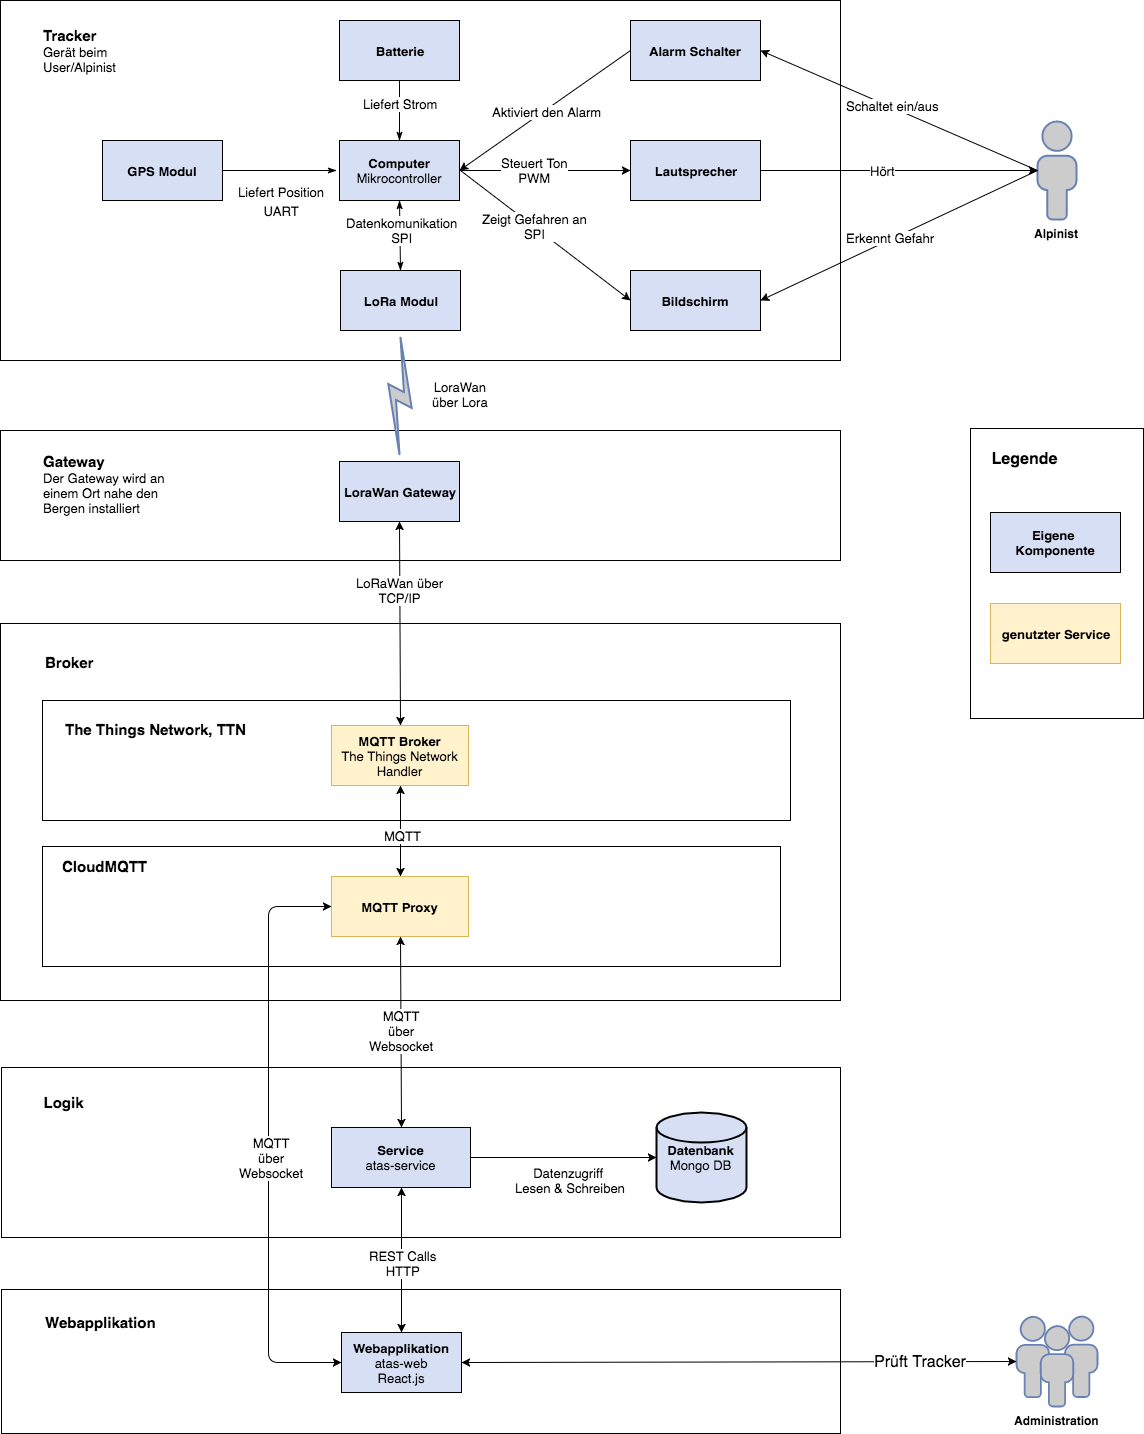
\includegraphics[width=\textwidth]{img/system/ATAS_SystemOverview_Detail_BA.png}
	\caption[Systemübersicht Detail]
	{Systemübersicht Detail}
\end{figure}
\newpage

\section{Tracker}
Wie in der untenstehenden Grafik ersichtlich, besteht der Tracker aus mehreren Komponenten/Modulen. Welche Komponenten verbaut und wie diese untereinander kommunizieren, wird im Kapitel 'Prototyp' genauer behandelt. Der Tracker besteht aus einem GPS Modul, einer Batterie, einem Notfallknopf, einem Lautsprecher, einem Display und einem Lora Modul.
\begin{figure}[H]
	\centering
	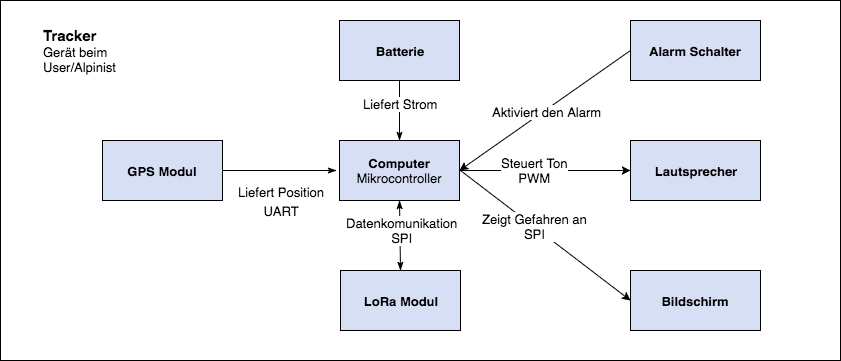
\includegraphics[width=\textwidth]{img/system/ATAS_SystemOverview_Tracker_BA.png}
	\caption[Tracker Detail]
	{Tracker Detail}
\end{figure}
\noindent
Die Komponenten haben die folgenden Funktionen und Aufgaben\\[0.3cm]
\textbf{Mikocontroller:} Steuert die Komponenten\\[0.3cm] 
\textbf{GPS Modul:} Ermittlung der Position des Trackers via GPS\\[0.3cm]
\textbf{Notfallknopf:} Aktiviert den Notfallmodus\\[0.3cm]
\textbf{Lora Modul:} Übermittelt die Positionsdaten per Lora und ob ein Notfall vorliegt. \\Empfang von Gefahrenzoneninformationen per Lora\\[0.3cm]
\textbf{Display:} Informiert den Alpinist über mögliche Gefahrenquellen\\[0.3cm]
\textbf{Lautsprecher: }Informiert den Alpinisten über mögliche Gefahrenquellen mittels Signalton

\newpage
\section{Gateway}
Der Gateway verbindet die Tracker mit dem TTN Netzwerk. Er sendet Daten zu den Trackern (Downlink) und empfängt Daten von den Trackern (Uplink). Was genau das TTN für eine Rolle übernimmt, wird später im Detail beschrieben.
\subsection{Diagramm}
\begin{figure}[H]
	\centering
	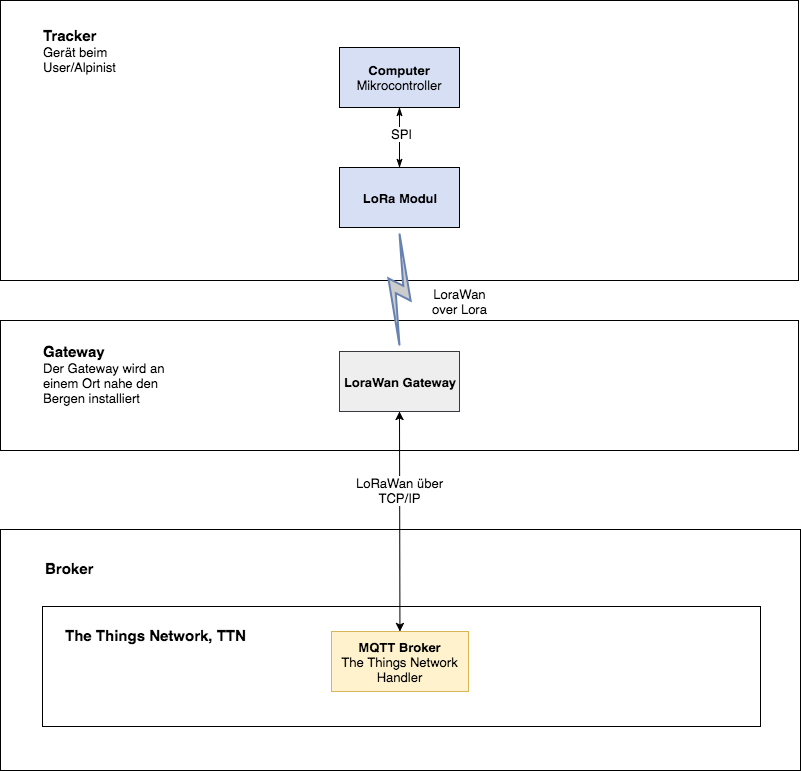
\includegraphics[width=\textwidth]{img/system/ATAS_SystemOverview_Detail_Gateway_BA.png}
	\caption[Gateway Detail]
	{Gateway Detail}
\end{figure}

\newpage
\section{Broker}
The broker has been split up in subcomponents. The broker service hasn’t been developed
by myself. I use two platforms the Things Network (TTN) and CloudMQTT.

\subsection{The Things Network (TTN)}
The Things Network short TTN is an internet platform whichs allows us to connect Lo-
RaWan devices. TTN will send (Downlink) and receive (Uplink) data from the trackers
via gateway. TTN will collect and store all the data which the gateways send to it. TTN
provies a MQTT Broker to access the data more easily.\\[0.3cm]
\textbf{Diagramm}
\begin{figure}[H]
	\centering
	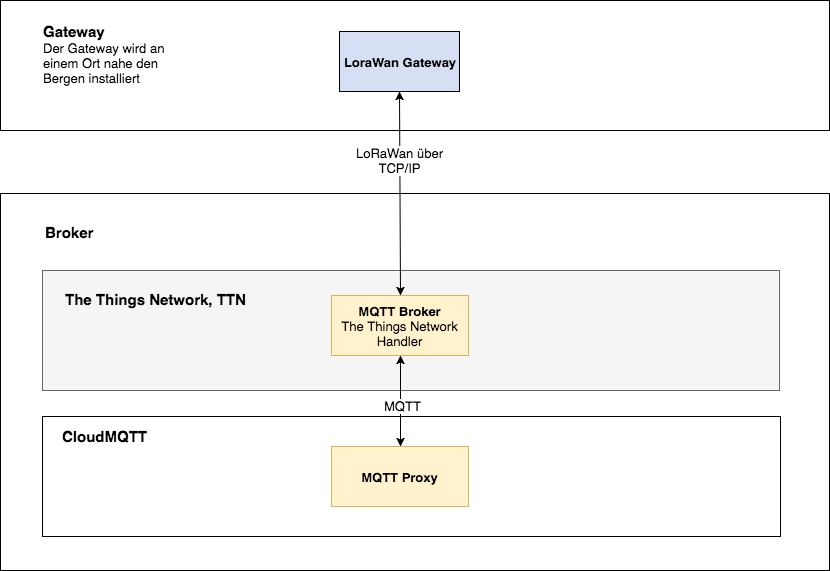
\includegraphics[width=\textwidth]{img/system/ATAS_SystemOverview_TTN_BA.png}
	\caption[TTN Detail]
	{TTN Detail}
\end{figure}

\newpage
\subsection{CloudMQTT}
Der MQTT Broker des TTN Netzwerkes bietet nur die Möglichkeiten die Daten via MQTT abzurufen. Ein Zugriff via MQTT über Websockets wird nicht unterstützt. Im Internet fand ich recht schnell den Service 'Cloud' MQTT.   CloudMQTT spiegelt den TTN MQTT Broker, bietet aber zusätzlich ein Websocket Interface. Atas-Web und Atas-Service können nun via CloudMQTT Daten an die Tracker senden und empfangen.\\[0.3cm]
Alle Daten welche zu CloudMQTT publiziert werden, werden nun auch automatisch zum TTN MQTT Broker publiziert (Published). Alle MQTT Topics welche vom CloudMQTT abonniert werden, werden auch vom TTN MQTT Broker abonniert (Subscribe).  \\[0.3cm]
\textbf{Diagramm}
\begin{figure}[H]
	\centering
	\includegraphics[width=0.9\textwidth]{img/system/ATAS_SystemOverview_CloudMQTT_BA.png}
	\caption[TTN Detail]
	{TTN Detail}
\end{figure}

\newpage
\section{Logik}
\subsection{Atas-Service}
TODO, PRIO 2

\newpage
\section{Webapplikation}
\subsection{Atas-Web}
TODO, PRIO 2

\chapter{Technologien}
\section{LoraWan}
Um das Projekt durchzuführen, musste ich mir mehr Wissen zum Thema LoraWan aneignen. Das im Projekt 2 aufgebaute System ist lauffähig, verwendet aber gewisse Standardeinstellungen welche ich einfach übernommen habe. Das Wissen, ob und wie man das System optimieren könnte ist nicht vorhanden.
\subsection{Begriffserklärung}
Zunächst ist es nötig einige Begriffe aus dem LoraWan Umfeld zu verstehen\\[0.5cm]
\begin{tabularx}{\textwidth}{ l|X }
	\textbf{Begriff} & \textbf{Erklärung} \\ \hline
	Endgerät & LoraWan Endgerät. Atas-Node ist ein LoraWan Endgerät.\\ \hline
	AppEUI& Eindeutige ID einer Applikation. 64Bit lang. Wird genutzt um ein Endgerät einer Applikation zuzuweisen.\\ \hline
	DevEUI& Eindeutige ID eines Endgerätes. \\ \hline
	DevAddr & Logische Geräte Adresse, analog einer IP Adresse in einem IP Netzwerk.\\ \hline
	NetSKey & Wird für die Verschlüsselung der Kommunikation zwischen Endgerät und Netzwerkanbieter bspw. TTN verwendet. Mittels Schlüssel kann die Datenintegrität sichergestellt werden d.H. Manipulierte Nachrichten werden erkannt.\\ \hline
	AppSKey & Mittels AppSKey werden die Nutzdaten separat nochmals verschlüsselt. Nur der Nutzer des Netzwerks kann die Daten lesen das Transportnetzwerk bspw. TTN kann diese nicht einsehen.\cite{ttnsecurity}\\ \hline
	Downlink & Kommunikation vom Gateway zu Endgerät\\ \hline
	Uplink & Kommunikation vom Endgerät zum Gateway
\end{tabularx}

\newpage
\subsection{Endgerät Verbindungsmethoden}
OTAA (Over-The-Air-Activation) und ABP (Activation By Personalization) sind Verbindungsmethoden für LoraWan Endgeräte in einem LoraWan Netzwerk.\cite{jaguar}. Die verwendete Methode definiert also wie sich ein Endgerät mit dem LoraWan Netzwerk verbindet. \\[0.3cm]
Die beiden Methoden bieten verschiedene Vor und Nachteile.

\subsubsection{ABP}
ABP ist das simplere aber \textbf{weniger sichere} Verfahren. Die Adresse DevAdr sowie die Schlüssel NetSKey und des AppSKey werden für jedes Endgerät \textbf{einmalig} generiert und fix auf dem Endgerät hinterlegt. Gelingt es einem Angreifer sich Zugang zum Endgerät zu verschaffen, kann er die Schlüssel stellen, ein zweites Gerät am Netzwerk registrieren, die Identität des Originals annehmen und damit die Daten verfälschen.\\[0.3cm]
Das Gerät muss sich nicht am Netzwerk anmelden. Das Endgerät kann direkt Daten senden. Empfängt ein Gateway die Daten, werden die Keys geprüft und die Kommunikation entsprechend an oder abgelehnt.

\subsubsection{OTAA}
Das Gerät muss sich am Netzwerk anmelden. Dieser Vorgang wird auch Join Prozedur genannt. Die DevAddr sowie die Keys NetSKey und AppSKey werden bei jeder Aktivierung des Gerätes \textbf{neu generiert} und an das Endgerät übertragen. Dieses Verfahren ist sicherer. Da es sich hier um eine bidirektionale Kommunikation handelt, müssen die Komponenten (Gateway \& Endgerät) Downlinks unterstützen.\\[0.3cm]
Das Installieren (Deployment) von Endgeräten wird vereinfacht. Das generieren vom AppSKey und NetSKey pro Endgerät entfällt. 

\newpage
\noindent
Die nachfolgende Grafik zeigt auf, wie der Kommunikationsaufbau via OTAA abläuft \cite{jaguar}.
\begin{figure}[H]
	\centering
	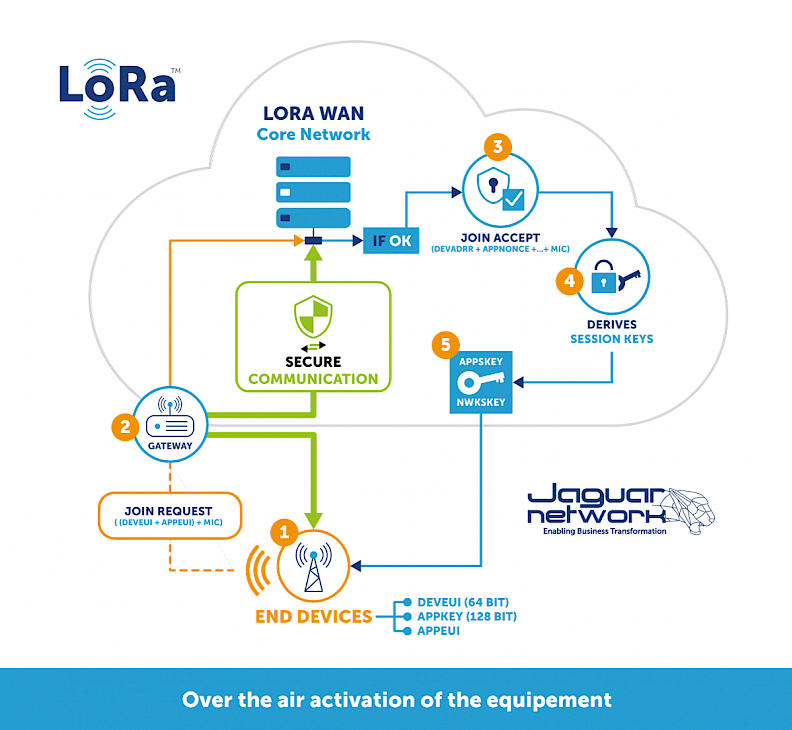
\includegraphics[width=0.9\textwidth]{img/otaa_schema.png}
	\caption[OTAA Ablauf]
	{OTAA Ablauf}
\end{figure}

\begin{enumerate}
	\item Gerät sendet einen Join Request.
	\item Die Gateways empfangen die Anfrage
	\item Das LoRaWan Netzwerk  bspw. TTN prüft die Angaben
	\item Session Keys werden generiert
	\item Keys werden an das Endgerät gesendet und für die zukünftige Kommunikation verwendet
\end{enumerate}

\newpage
\subsubsection{Schlussfolgerung}
Obschon die Sicherheit während diesem Projekt nicht im Vordergrund steht, ist es sicher zukunftsorientierter direkt OTAA einzusetzen. Systeme welche zum Schutz von Personen eingesetzt werden, müssen so sicher wie nur möglich konzeptioniert sein.\\[0.3cm]
Sowohl Endgerät als auch Gateway unterstützen Downlinks, damit gibt es keine technische Hürde der den Einsatz von OTAA verhindern würde. Aus diesem Grund habe ich während dem Projekt die Verbindungsmethodik von ABP auf OTAA umgestellt und konnte damit die Sicherheit des Systems verbessern.

\subsection{Frame Counters}
Ein Endgerät besitzt zwei Zähler (FCntUp, FCntDown). Die Zähler werden bei einer Downlinkmessage (FCntDown) resp. Uplinkmessage (FCntUp) erhöht (+1).\\[0.3cm]
Wird eine Reply Attacke durchgeführt d.H. ein Paket nochmals gesendet, wird dieses Paket vom System verworfen. Dies geschieht deshalb, weil das System bereits eine Nachricht mit dem gleichen Framecounter erhalten hat.\\[0.3cm]
Diese zusätzliche Information wird mir beim Testen der Übertragung überaus nützlich sein. Anhand der Nummerierung, kann sehr schnell erkannt werden, ob ein Paket nicht sauber empfangen werden konnte. Bspw. Erhalten wir die Pakete 4,5,7 $\rightarrow$ Paket 6 wurde nicht korrekt übertragen.

\subsection{Adaptive Data Rate (ADR)}
Ist Adaptive Data Rate aktiv (ADR), entscheidet das LoraWan Endgerät selbständig ob und wie die Kommunikation optimiert werden soll. Gemäss TTN \cite{ADRTTN} sollte ADR nur für statische Nodes oder für mobile Nodes zur Erkennung von Stops (keine Bewegung) verwendet werden. Gemäss TTN ist ADR also nicht unbedingt für die Atas-Tracker geeignet. Die Tracker sind ja meistens in Bewegung bspw. durch Laufen, Ski fahren usw. Dennoch wurde mein Interesse geweckt und ich wollte genauer wissen warum dieses Feature nicht empfohlen wird.\\[0.3cm]
Sobald ein LoraWan Endgerät dem Netzwerk mitteilt, dass es ADR verwenden möchte, beginnt das TTN Daten aufzuzeichnen. Die letzten 20 Messdaten die der Node gesendet hat werden analysiert. Es folgt ein Beispiel von der TTN Webseite:


\chapter{Prototyp}
Das Bachelorarbeit wird in 2 Hauptaufgaben aufgeteilt.\textbf{ Testing} und das erstellen eines zweiten Prototyps nachfolgend genannt \textbf{Prototyp 2}. Dieses Kapitel beschreibt, wie ich beim Aufbau des Prototypen 2 vorgegangen bin.

\section{Begründung neuer Prototyp}
Es gibt diverse Gründe für diesen Schritt
\begin{enumerate}
	\item Auf dem Prototyp 1 wird ein vollwertiges Betriebssystem (Raspian, Linux Derivat) eingesetzt. Einige Funktionen bspw. das Lesen der GPS Daten werden vom System sehr vereinfacht. Dies ermöglichte mir einen raschen und unkomplizierten Aufbau der Software. Obschon ein solches 'High Level' OS eine grosse Hilfe in der Entwicklung darstellt, ist es in der Industrialisierung der Lösung eher hinderlich. Der Einsatz eines OS hat diverse Nachteile
	\begin{itemize}
		\item Vom OS selbst benötigen wir für den Betrieb der Atas-Node Software nur einen Bruchteil der Funktionalität. Speicher, Memory und Systemperformance wird für Systemprozesse verschwendet. 
		\item Durch die hohe Auslastung des Systems werden stärkere Prozessoren benötigt. Der Energieverbrauch der Lösung steigt.
		\item Mehr Software bedeutet Zwangsläufig mehr Fehlerquellen. Obschon das eingesetzte System (Raspian) als Stabil gilt, kann es aufgrund der Softwarekomplexität zu Fehlern kommen.
		\item Durch den Einsatz eines OS reduzieren wir die Sicherheit des ganzen Systems. Je mehr Interfaces ein System anbietet, desto anfälliger wird es für den unerlaubten Zugriff.
	\end{itemize}
	\item Der Prototyp 1 bietet und viele Anschlussmöglichkeiten. Bspw. für ein Display, USB, oder eine RJ45 Buchse. Funktionen die wiederum welche Entwicklung stark vereinfachen, aber den Energieverbrauch erhöhen und die Grösse des Systems unnötig vergrößert. 
	\item Die Verbauten Komponenten sind nicht für eine Industrialisierte Lösung geeignet. Man könnte sogar von einem 'Bastelprojekt' sprechen. Die Komponenten hindern das Projekt daran eine professionelle Form anzunehmen.
\end{enumerate}

\section{Ablauf Prototyping}
Aus meiner Sicht bildet während der Arbeit zu konstruierende Prototyp 2 nur einen Zwischenschritt bis zu Finalen Version. Eine Visualisierung meiner Vorstellung:\\
\begin{figure}[H]
	\centering
	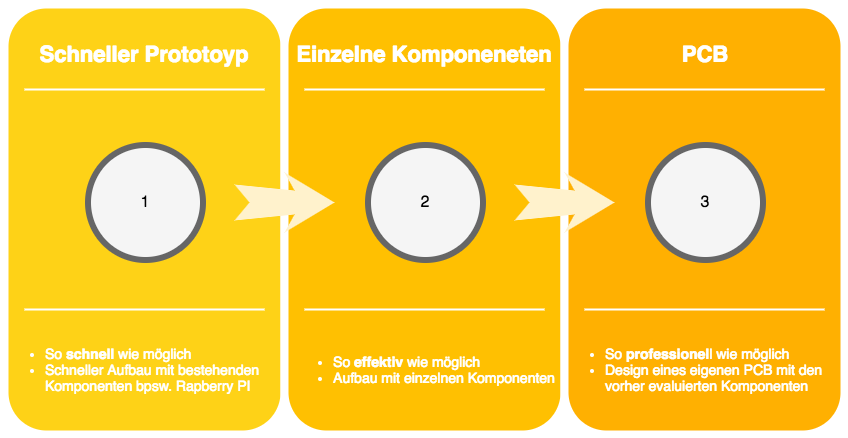
\includegraphics[width=\textwidth]{img/projectFlow_Prototype.png}
	\caption[Prototyping Ablauf]
	{Prototyping Ablauf}
\end{figure}
\noindent
Mein Ziel ist es mit dem Umstieg auf anderen Komponenten, den Grundstein für den Prototypen 3 zu legen. Der Prototyp 3 ist nicht Bestandteil dieser Arbeit. Prototyp 3 bildet die finale Prototyp Version. Die Einzelnen Komponenten vom Prototyp 2 werden auf einen eigens designeten PCB installiert. Durch diesen Schritt würde sich das System in Sachen Platzbedarf nochmals massiv verbessern.

\newpage
\section{Ablauf Vorgehen}
Der im Projekt 2 erstellte Prototyp wurde mit sehr simplen vorgefertigten Elektronikkomponenten umgesetzt. Ziel dieser Arbeit war es in möglichst kurzer Zeit einen Prototypen aufzubauen. Während dieser Arbeit sollen nun neue Komponenten evaluiert und ein zweiter Prototyp erstellt werden. Der Ablauf dieser Phasen sieht wie folgt aus:\\[0.3cm]

\begin{figure}[H]
	\centering
	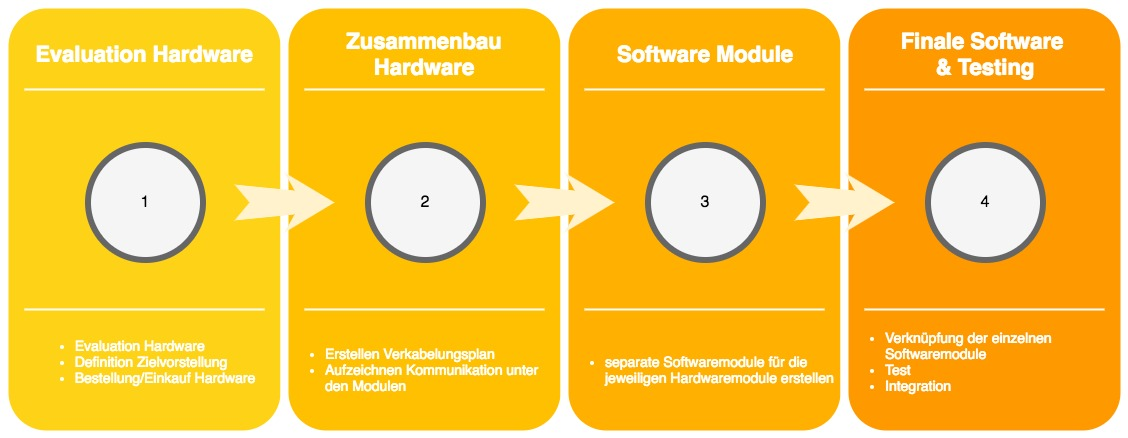
\includegraphics[width=\textwidth]{img/projectFlow_hardware.jpg}
	\caption[Flowchart Prototyp 2]
	{Ablauf für den Aufbau des zweiten Prototyps}
\end{figure}
\noindent
Die einzelnen Schritte werden auf den kommenden Seiten detailliert erklärt.

\newpage
\section{Evaluation Hardware}
Auf Grundlage der bestehenden Prototyps soll neue Hardware evaluiert werden. Der Funktionsumfang des Prototyps soll gleichwertig bleiben. Sind die Komponenten erst definiert, wird das Material bestellt.\\
Für den Aufbau des zweiten Prototypen wurde die nachfolgende Hardware verwendet.\\[0.5cm]
\begin{tabularx}{\linewidth}{XXX}
		\textbf{Gerätetyp} & \textbf{Model} & \textbf{Bild} \\ \hline
		Entwicklungsboard & \makecell[l]{Espressfif ESP-WROOM-32\\ Core Dev Kit}  & \parbox[c]{1em}{
			\vspace{8pt}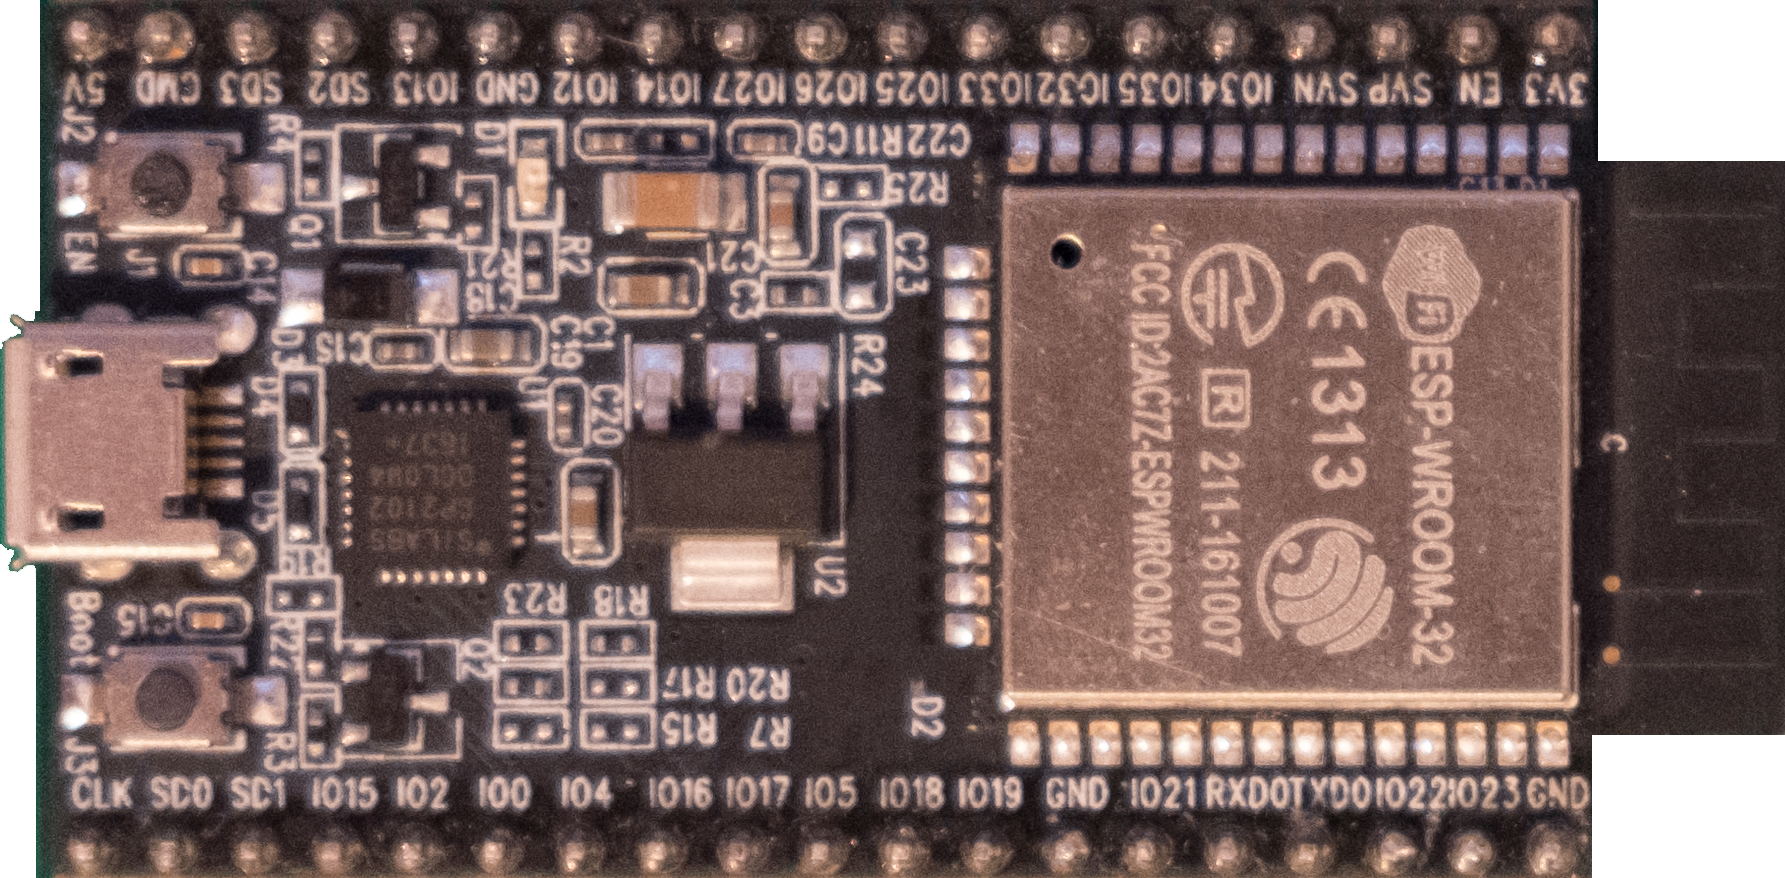
\includegraphics[width=0.3\textwidth]{img/system/esp32.png}\vspace{8pt}} \\ \hline
		GPS Module& ublox Neo 6M & \parbox[c]{1em}{
			\vspace{8pt}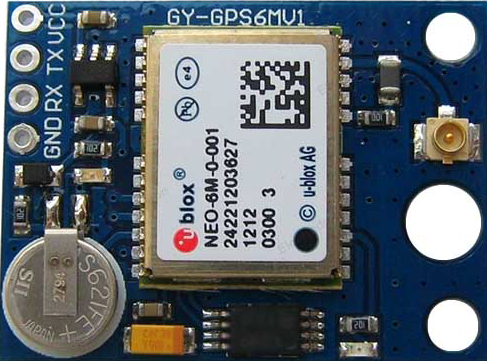
\includegraphics[width=0.3\textwidth]{img/system/gps.png}\vspace{8pt}} \\ \hline
		Lora Modul & RFM96 & \parbox[c]{1em}{
			\vspace{8pt}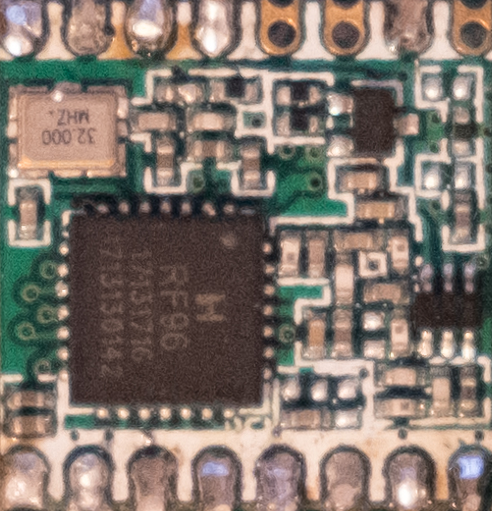
\includegraphics[width=0.18\textwidth]{img/system/lora.png}\vspace{8pt}} \\ \hline
		Speaker & Piezo Speaker  & \parbox[c]{1em}{
			\vspace{8pt}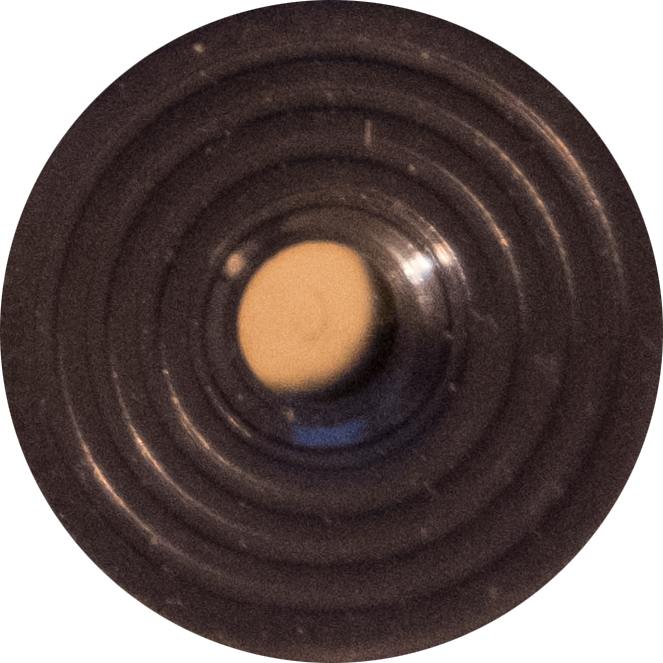
\includegraphics[width=0.15\textwidth]{img/system/speaker.png}\vspace{8pt}} \\ \hline
		Display & \makecell[l]{eink Display Waveshare \\ 1.54  Zoll 200x 200}  &\parbox[c]{1em}{
			\vspace{8pt}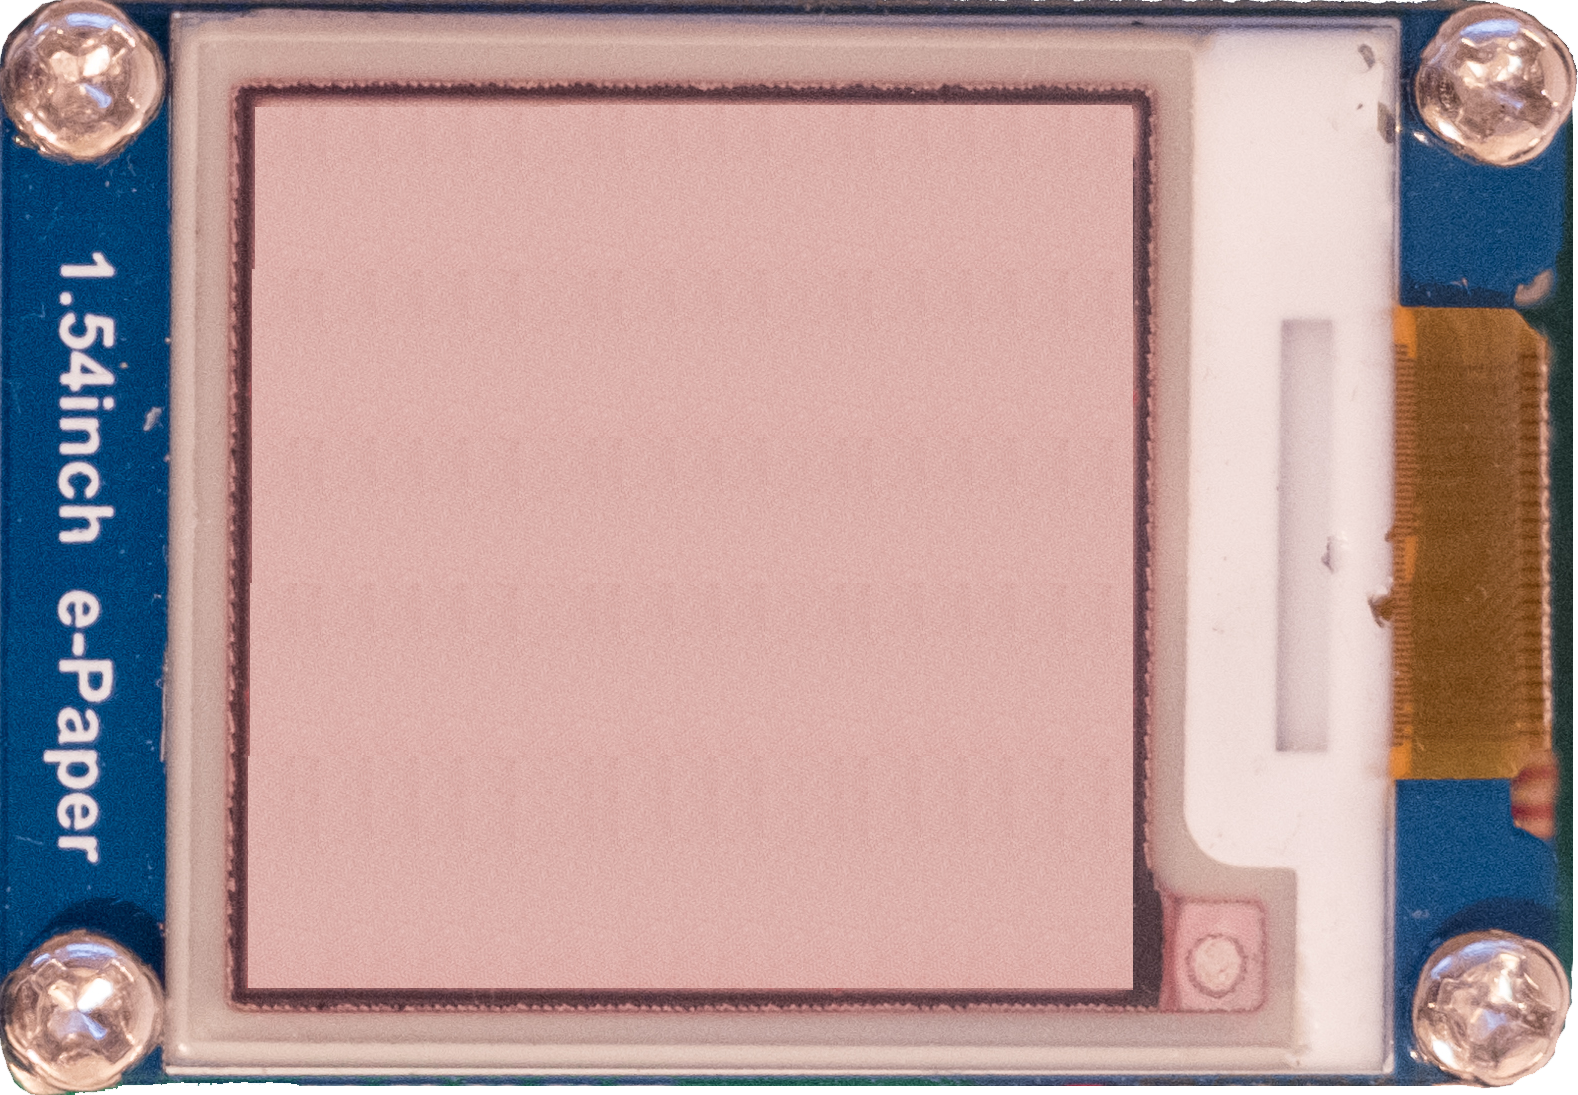
\includegraphics[width=0.3\textwidth]{img/system/display.png}\vspace{8pt}} \\ \hline
		Schalter & gewöhnlicher 4 Pin Schalter & \parbox[c]{1em}{
			\vspace{8pt}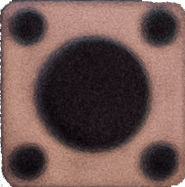
\includegraphics[width=0.07\textwidth]{img/system/schalter.png}\vspace{8pt}} \\ \hline
\end{tabularx} 
\noindent
Aus Zeitgründen habe ich mich bei den Komponenten von bestehenden Projekten resp. Einträge im Internet inspirieren lassen. Es gab kein spezielles Auswahlverfahren für die restlichen Komponenten. Meiner Meinung nach nicht das beste Vorgehen. Bei einem erneuten Projekt in dieser Richtung müsste ich vorher die Kriterien für die Komponenten festlegen.
\newpage
\subsection{Lora-Antenne}
Ich beging den Fehler, anzunehmen, dass beim Kauf des Lora-Moduls eine Antenne mitgeliefert wird. Da ich über sehr wenig Erfahrungen in der Telekommunikationswelt verfügte, wollte ich mich auch mit diesem Thema etwas genauer befassen. Ich entschied mich gegen eine erneute Bestellung und baute mir die Antenne einfach selbst. Nach einer kurzen Internetrecherche fand ich heraus wie mit einfachen Mitteln eine zuverlässige Antenne für 868Mhz gebaut werden kann \cite{wavelengthTTN}. Ein einfaches Kabel genügt. Das Kabel muss die Länge der Wellenlänge oder einen Bruchteil bspw. 1/2 oder 1/4 der Wellenlänge haben. Die Berechnung der Wellenlänge ist mit der nachfolgenden Formel möglich \cite{wavelength}.\\[0.3cm]
Es gilt $\lambda$ = Wellenlänge, v = Übertragungsgeschwindigkeit (Lichtgeschwindigkeit), f = Durchschnitt der Frequenz (Lora Frequenz in Europa)
\begin{center}
	\begin{eqnarray*}
		\lambda &=& \frac{v}{f}\\
		\lambda &=& \frac{299.792.458 m/s}{868.000.000} = 34,54cm\\
		\frac{\lambda}{2} &=& \frac{34,53cm}{2} = 17,27cm\\
		\frac{\lambda}{4} &=& \frac{17,27cm}{2} = 8,63cm \\
	\end{eqnarray*}
\end{center}
17,27cm sind für meinen Prototypen zu lange. Ich entschied mich 1/4 der Wellenlänge zu verwenden. Für eine Antenne musste also nur ein Kabel mit der Länge \textbf{8.63cm} vorbereitet und mit dem Antennenport des Lora Moduls verbunden werden.\\[0.3cm]
Das Resultat\\
TODO BILD\\[0.3cm]
Die Kommunikation funktioniert einwandfrei und ist mit der des ersten Prototypen vergleichbar. Mir ist bewusst, dass der Empfang mit einer professionellen Antenne noch besser werden würde. Die Thematik 'Antenne' müsste bei einer Weiterführung des Projektes nochmals beleuchtet werden.
\newpage
\section{Zusammenbau Hardware}
Die Komponenten werden zusammengebaut und untereinander verbunden. Zur besseren Übersicht wird ein Schema  der Elektronik erstellt.
\subsection{Schema}
Die Kommunikation unter den Komponenten wurde im Laufe der Projektarbeit  für mich immer unübersichtlicher. Um mir die Arbeit zu erleichtern, habe ich ein Schema mit den Komponenten erstellt. Vor der Arbeit hatte ich noch nie ein Schema gezeichnet und musste mich zuerst einige Stunden in die Materie einarbeiten. Auf anraten einiger Kollegen, mit Erfahrung im Elektronik Umfeld, sowie der frei verfügbaren Lernressourcen und Vorlagen, fiel meine Wahl auf das Programm \textbf{Eagle} der Firma Autodesk \cite{autodesk}. Dank der guten Dokumentation und den Lernvideos auf diversen Plattformen bspw. Youtube kam ich beim Zeichnen schnell vorwärts. \\[0.3cm] 
Ich begann damit Vorlagen der Elektronischen Bausteine/Chips finden. Die Vorlagen zu Lora, GPS, ESP, Schalter und Piezo Lautsprecher konnte ich teilweise vom Hersteller oder von der Community herunterladen und in Eagle importieren. Für das Display musste ich ein bestehende Vorlage eines Displays anpassen. Ich habe dabei die Größe und die Pinbelegung verändert, damit das Element wie das verwendete Display (Waveshare eInk 200x200) aussieht. \\[0.3cm]
Das Schema ist auf der nachfolgenden Seite abgebildet.
\newpage

\begin{figure}[H]
	\centering
	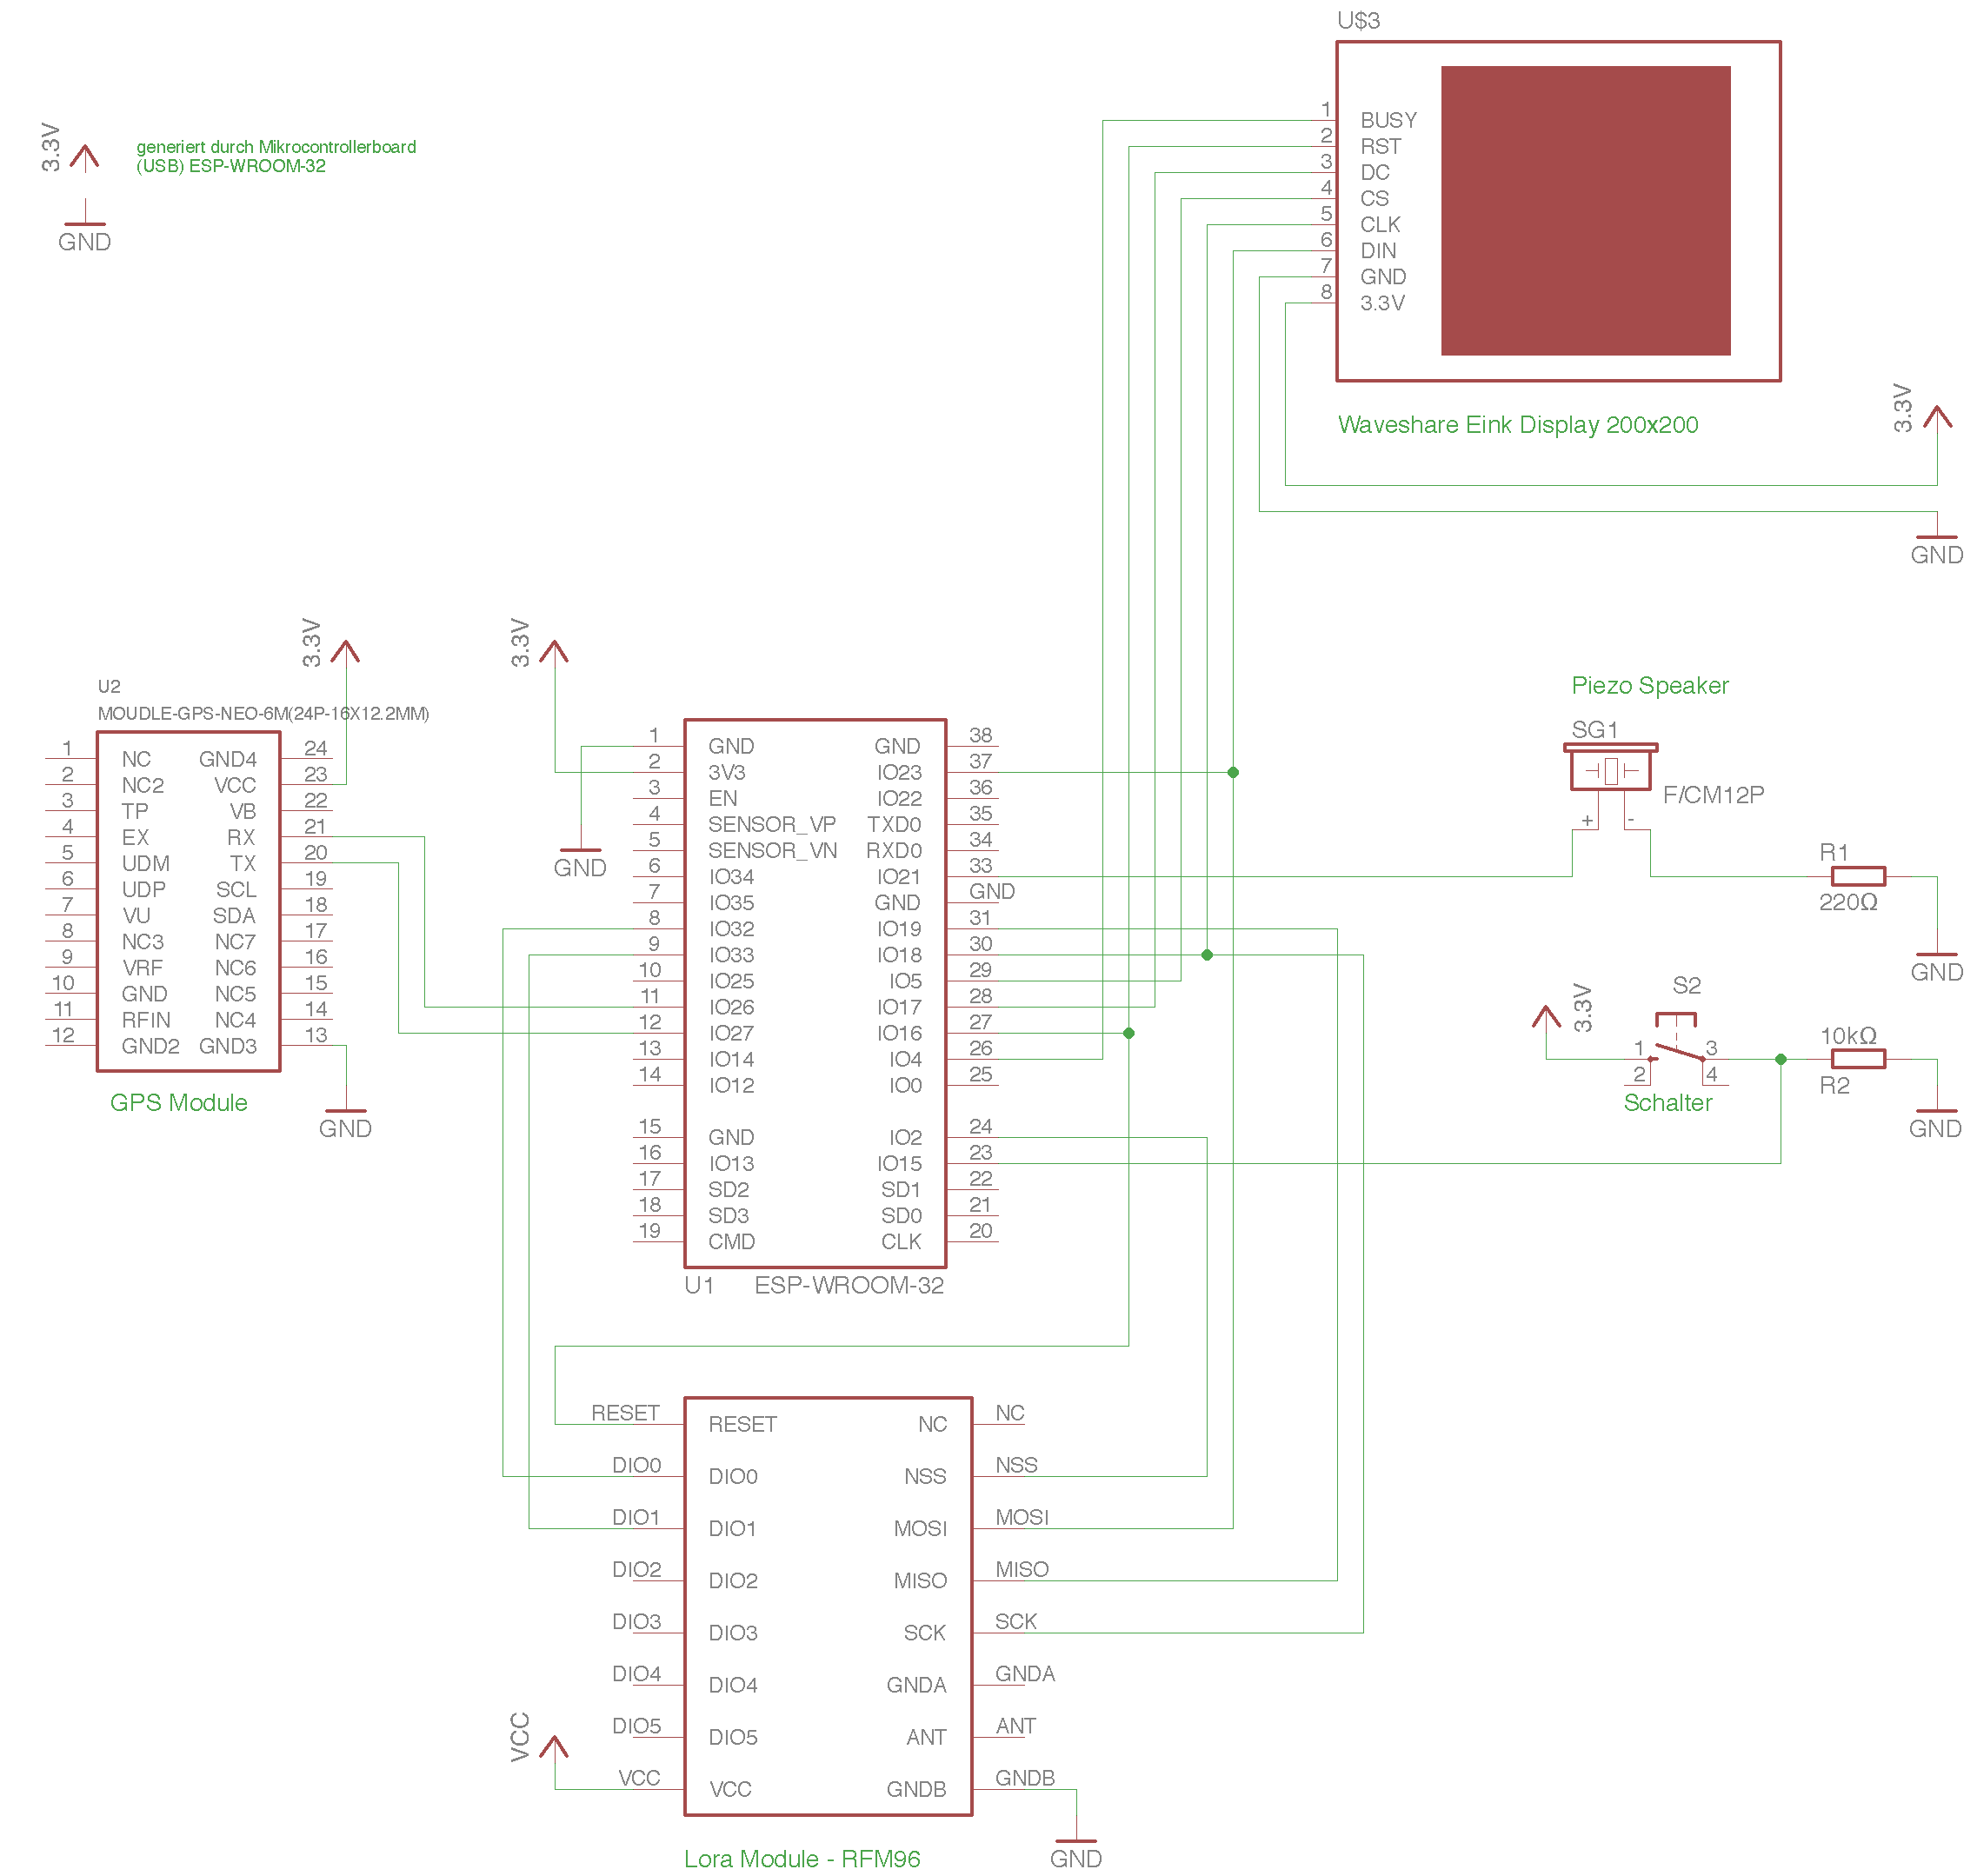
\includegraphics[width=\textwidth]{img/prototyp_schema.png}
	\caption[Prototyp2 Schema]
	{Prototyp 2 Schema}
\end{figure}

\newpage
\subsection{Mikrocontroller - Pinbelegung}
Die nachfolgende Pinbelegung wurde verwendet um den ESP32 mit den übrigen Komponenten zu verbinden. Zu meiner Überraschung sind die Pins nicht fix durch den ESP32 festgelegt. Die Pins können meist für jegliche Funktion bspw. PWM, SPI verwendet werden. Durch diese Freiheit wird die Verkabelung massiv vereinfacht und die Anzahl der möglichen Fehlerquellen wird reduziert.\\
\begin{tabularx}{\textwidth}{ l|l|X }
	\textbf{MCU Pin} & \textbf{Modul} & \textbf{Funktion}\\ \hline
	IO02 & Lora & SPI ChipSelect (CS)\\\hline
	IO04 & Lora + Display& SPI Busy\\ \hline
	IO05 & Displayl& SPI ChipSelect(CS)\\\hline
	IO15 & Switch & -\\ \hline
	IO16 & Lora + Display & SPI Reset\\\hline
	IO17 & Display&  DataCommand (DC)\\ \hline
	IO18 & Lora + Display & SPI Clock (CLK)\\ \hline
	IO19 & Lora + Display & Master In Slave Out (MISO) \\\hline
	IO21 & Piezo Speaker & - \\ \hline
	IO23 & Lora + Display & SPI Master Out Slave In (MOSI) \\\hline
	IO26 & GPS & UART RX\\ \hline
	IO27 & GPS & UART TX\\ \hline
	IO32 & Lora & DIO0\\ \hline
	IO33 & Lora & DIO1\\ \hline
\end{tabularx}

\section{Kommunikation}
In der nachfolgenden Übersicht wird die Kommunikationsart zwischen den Komponenten aufgezeigt.\\
\begin{figure}[H]
	\centering
	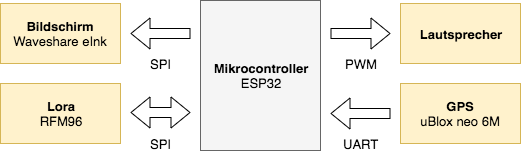
\includegraphics[width=\textwidth]{img/system/ATASNode2_Kommunikation.png}
	\caption[Kommunikationsart Prototyp 2]
	{Kommunikationsart Prototyp 2}
\end{figure}


\newpage
\subsection{Zusammenbau}
Die Komponenten wurden auf einer Entwicklungsplatine (PCB Breadboard) platziert und verlötet resp. angeschraubt. Der Mikrocontroller wurde absichtlich nicht im Zentrum platziert, damit der Zugang zum USB Anschluss frei blieb. Abschließend wurde gemäß Schema die Komponenten untereinander verkabelt.\\
\begin{figure}[H]
	\centering
	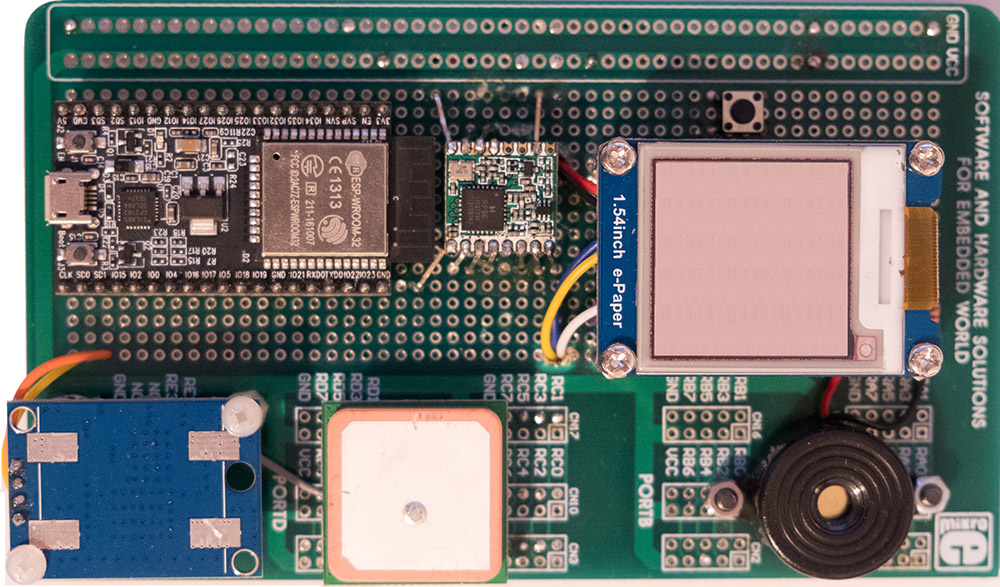
\includegraphics[width=\textwidth]{img/system/prototyp2.jpg}
	\caption[Prototyp 2]
	{Prototyp 2}
\end{figure}

\newpage

\section{Software Module}
Der bestehende Sourcecode des Prototyps 1 kann leider nicht eins zu eins übernommen werden. Die Software ist sehr stark für die Raspberry Pi Umgebung angepasst und ist daher nicht mit dem ESP32 Umfeld kompatibel. Die Software muss portiert werden. Die Logik der Software kann übernommen werden.\\[0.3cm]
Pro Hardware Modul wird ein separates Software Modul erstellt.

\subsection{Entwicklungsumgebung}
Duch den Umstieg vom Rapberry Pi auf den Mikrocontroller ESP32 hat sich im Bereich der Entwicklungsumgebung einiges verändert. Die ESP32 Plattform unterstützt, Stand heute (16.11.2017), zwei Entwicklungsumgebungen. Das wäre einerseits ESP-IDF (IoT Development Framework) sowie Arduino\cite{espidfarduino}. Die beiden Umgebungen sind miteinander kombinierbar. So kann in der IDF Umfeld die Arduino Unterstützung als Komponente importiert werden. Bestehende für Arduino konzipierte Bibliotheken können dadurch ebenfalls verwendet werden. Ich habe mich in Absprache meines Betreuers für die ESP-IDF Umgebung entschieden und mein System entsprechend vorbereitet. Die Installation der Entwicklungsumgebung ist nicht schwer, bedingt aber einige manuelle Schritte. Die Umgebung besteht aus einer Reihe von Tools (Toolchain) zum Kompilieren, Fehlersuche und dem Flashen des Mikrocontrollers.\\[0.3cm]
Ich verzichte an dieser Stelle auf eine detaillierte Auflistung aller Installationsschritte. Die Installation wurde gemäss der Anleitung auf der Webseite der Firma Espressif durchgeführt \cite{espidfinstallation}.\\[0.3cm]
Als Hostsystem wurde ein macOS System verwendet. Damit das System den ESP korrekt erkennen konnte, musste ein zusätzlicher Treiber installiert werden \cite{espidfdriver}. 

\subsection{Display}

\newpage
\section{Finalisierung}
Die Erstellten Softwaremodule werden miteinander verknüpft und die Software fertiggestellt. Abschließend werden einige Testszenarien durchgeführt. 

\chapter{Testing}
\section{Ablauf Vorgehen}
Ein Teil des Systemaufbaus aus dem vorgängigen Projekt soll getestet werden. In diesem Kapitel wird genau beschrieben, wie beim Testing des Systems vorgegangen wird.\\[0.3cm]
In der nächsten Abbildung sind die geplanten Schritte aufgeführt.
\begin{figure}[h]
	\centering
	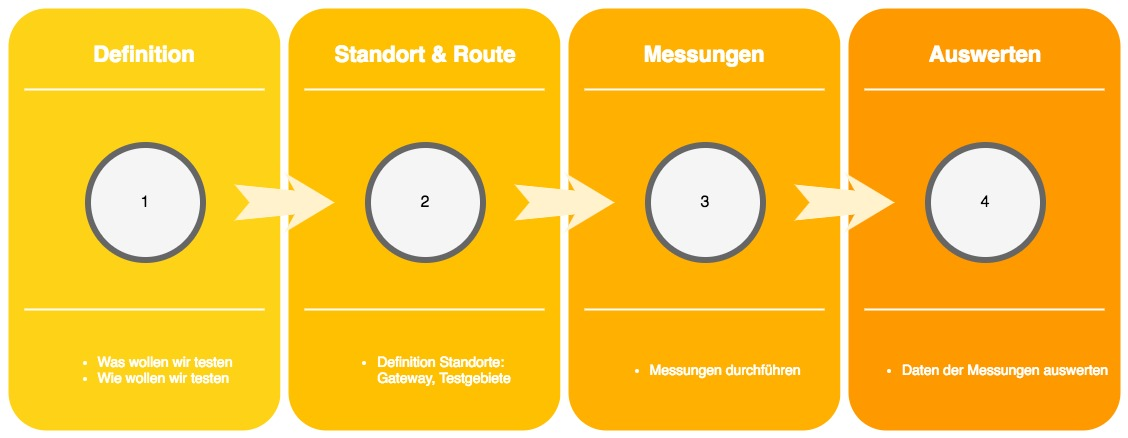
\includegraphics[width=\textwidth]{img/projectFlow_testing.jpg}
	\caption[Flowchart Testing]
	{Ablauf Testing}
\end{figure}
\\ 
Die einzelnen Schritte werden auf den kommenden Seiten detailliert erklärt.
\newpage
\section{Definition}
Es muss definiert werden
\begin{itemize}
	\item welche Komponenten geprüft werden sollen\\[0.3cm]
	Während der Arbeit soll die Kommunikation zwischen Atas-Node und Atas-Gateway getestet werden.
	\item welche Aspekte der Komponente sollen betrachtet werden\\[0.3cm]
	Der Fokus liegt auf der \textbf{Zuverlässigkeit} der Übertragung. Mich interessiert, wie sicher es ist, dass eine Meldung ihr Ziel erreicht. 
	\item mit welchen Mitteln resp. Messinstrumenten gemessen wird\\[0.3cm]
	Das TTN Netzwerk bietet uns die Möglichkeit mittels Dashboard einzusehen, wann welche Pakete auf dem Gateway eintreffen. So können wir prüfen ob die Verbindung zwischen Gateway und Tracker funktioniert.\bigskip
	
	\begin{minipage}{\linewidth}
		\centering
		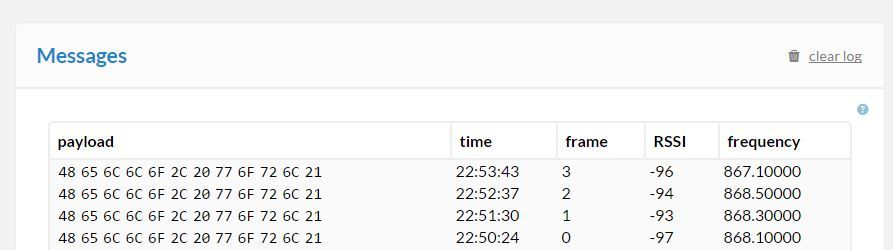
\includegraphics[width=\linewidth]{img/ttn_messages}
		\captionof{figure}{TTN Messages}
	\end{minipage}
	
	\item welche Daten sollen untersucht werden\\[0.3cm]
	Für die Messungen sind mehre Daten von Interesse. Dazu gehören 
	\begin{itemize}
		\item Signalstärke
		\item Wie viele Pakete gehen verloren
		\item Distanz der Übertragung
		\item Sichtverhältnisse zwischen Sender und Empfänger
	\end{itemize}
\end{itemize}

\subsection{Schlussfolgerung}
Abgeleitet aus der vorhergehenden Definitionen ergibt sich die folgende Aufgabenstellung im Bereich Testing. Es muss eine Testumgebung aufgebaut und die Verbindung getestet werden. Um von den bestehenden TTN Gateways unabhängig zu sein, wird ein \textbf{eigener Gateway} aufgebaut. Anschließend werden mehrere Wanderungen auf verschiedenen Routen durchgeführt. Die Verbindung wird aufgebaut und mittels TTN Dashboard geprüft.

\newpage
\section{Standort}
Ausgehend von den vorangegangen Definitionen muss folgendes definiert werden.
\begin{itemize}
	\item Es muss ein Ort gefunden werden, wo der Gateway platziert werden kann.\\[0.3cm]
	Der Standort kann frei gewählt werden. Zwei Kriterien müssen zwingend erfüllt sein. 
	\begin{enumerate}
		\item
		Der Gateway empfängt die Daten der Endgeräte und muss diese dem TTN Netzwerk über das Internet weiterleiten können. Eine stabile Internetverbindung ist nötig. 
		\item 
		Der Standort sollte in der nähe von möglichen Wanderrouten resp. Testbereichen liegen.
	\end{enumerate}
	\item Für die Tests sollten mind. 3 Routen/Wanderungen definiert werden. Dies garantiert eine vernünftige Anzahl an Messwerten.
	\item Auf dem Pfad selbst werden mind. 5 Orte definiert wo die Verbindungstests durchgeführt werden.
\end{itemize}

\newpage
\subsection{Gateway}
Der Standort für den LoRa Gateway war schnell gefunden. Ich arbeite momentan als Informatik Systemengineer bei der Hoffmann Neopad AG. Die Firma besitzt eine Niederlassung in der Nähe der Stadt Thun (BE). Das Gebäude ist 2 Stockwerke hoch und die Adresse liegt in unmittelbarer nähe der Voralpen. Hohe Berge für einen möglichen Testlauf sind max. 20km entfernt. Dazu zählen beispielsweise das Stockhorn, Niesen sowie das Niederhorn.\\[0.1cm]
\begin{tabularx}{\textwidth}{ l|X }
		\textbf{Beschreibung} & \textbf{Bild} \\ \hline
		Standort Hoffmann Neopac AG & \parbox[c]{1em}{
			\vspace{8pt}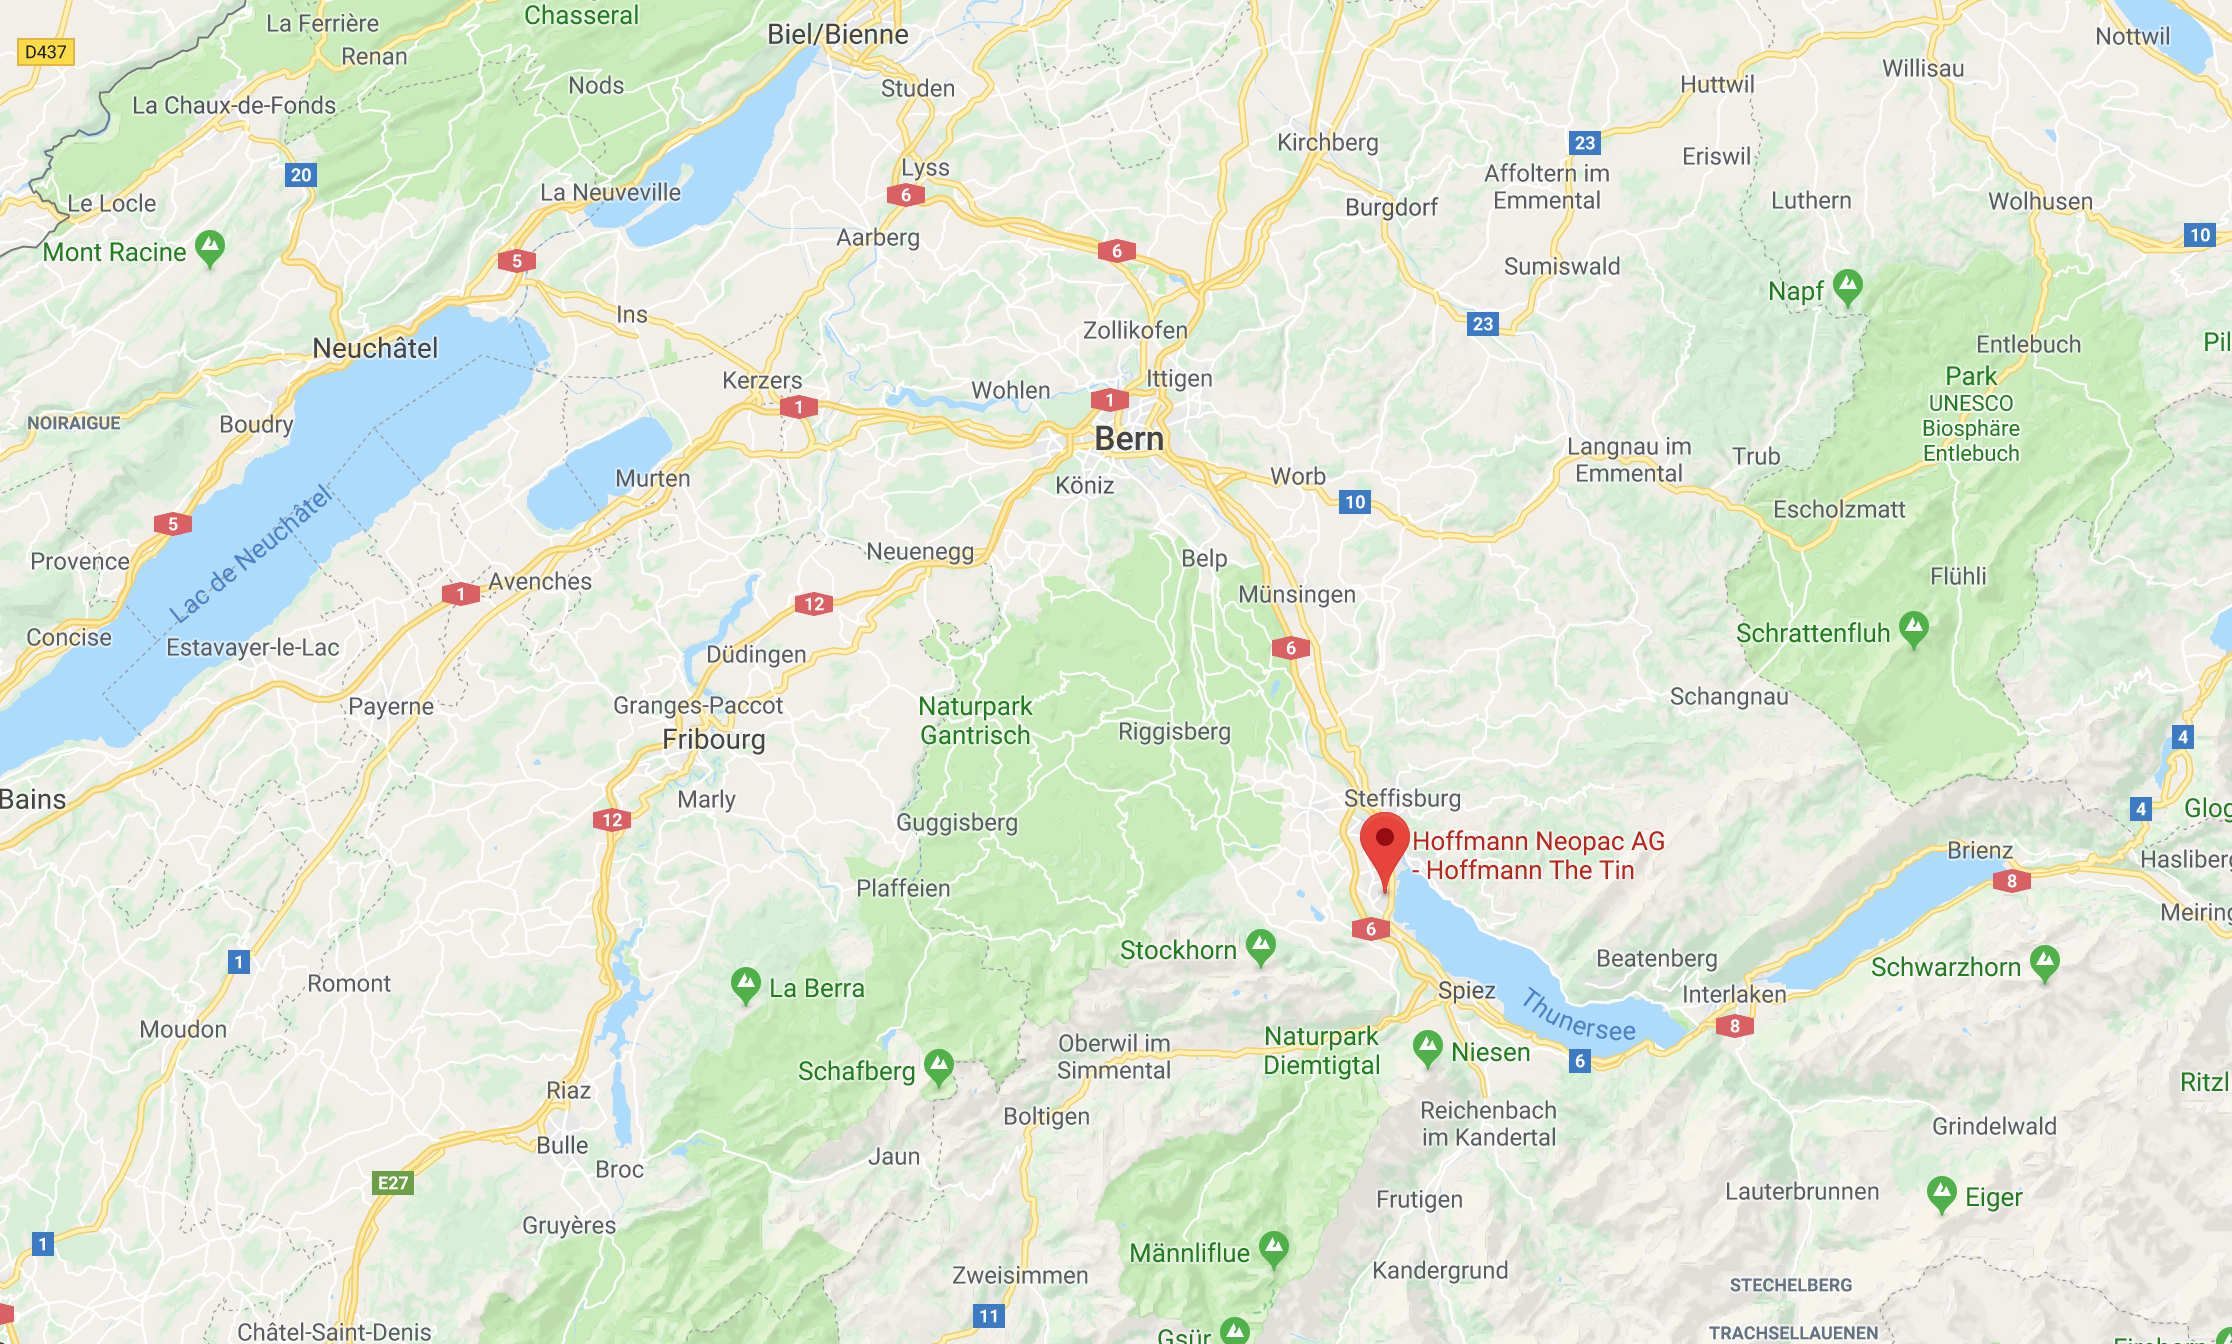
\includegraphics[width=0.6\textwidth]{img/gateway/gateway_map.png}\vspace{8pt}} \\ \hline
		Standort Gateway auf Gebäude &  \parbox[c]{1em}{
			\vspace{8pt}\includegraphics[width=0.6\textwidth]{img/gateway/gateway_building_front.jpg}\vspace{8pt}} \\ \hline
\end{tabularx}

\newpage
\subsection{Testregionen}
Im ersten Teil meiner Arbeit konzentrierte ich mich stark auf den Aufbau des Prototypen. Das Testing hatte für mich eher eine kleinere Priorität. Ein Fehler wie sich später herausstellen sollte. Der Winter ließ, wie sonst nicht üblich, nicht lange auf sich warten. Bereits Mitte Oktober beginn es zu schneien. Wanderrouten welche ich für das Testing verwenden wollte, bspw. der Nordaufstieg Stockhorn, wurden wegen zu hoher Lawinengefahr geschlossen.\\[0.3cm]
Nichtsdestotrotz konnte ich 2 Testregionen definieren, welche einfach zugänglich und soweit gefahrlos passierbar waren.
\begin{tabularx}{\textwidth}{ l|X }
	\textbf{Niederhorn} & \textbf{Bild} \\ \hline
	Region &  \parbox[c]{1em}{
		\vspace{8pt}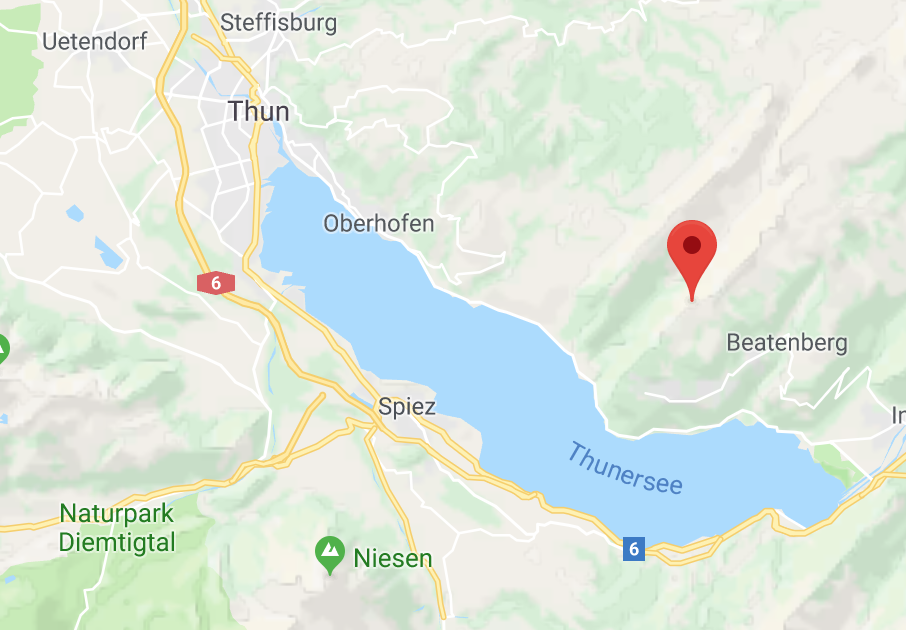
\includegraphics[width=0.6\textwidth]{img/testregions/niederhorn.png}\vspace{8pt}} \\ \hline
	Höhenunterschied zum Gateway&\parbox[c]{1em}{
		\vspace{8pt}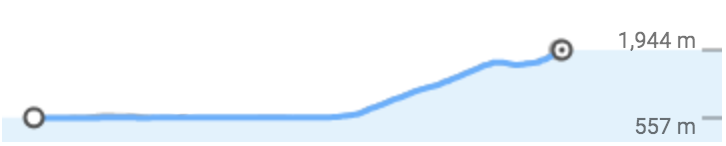
\includegraphics[width=0.6\textwidth]{img/testregions/niederhorn_altitude.png}\vspace{8pt}} \\ \hline
\end{tabularx}

\newpage
\begin{tabularx}{\textwidth}{ l|X }
	\textbf{Heiligenschwendi} & \textbf{Bild} \\ \hline
	Region & \parbox[c]{1em}{
		\vspace{8pt}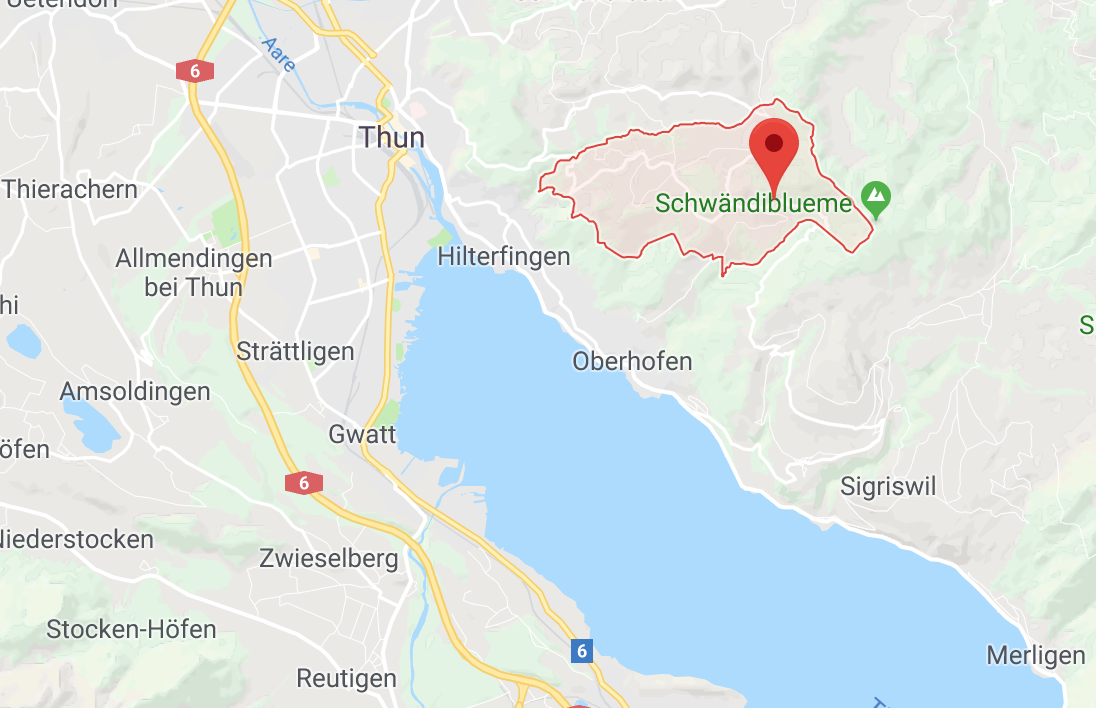
\includegraphics[width=0.6\textwidth]{img/testregions/heiligenschwendi.png}\vspace{8pt}} \\ \hline
	Höhenunterschied zum Gateway&\parbox[c]{1em}{
		\vspace{8pt}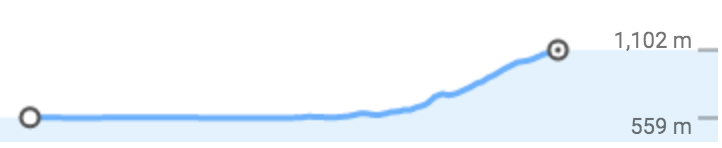
\includegraphics[width=0.6\textwidth]{img/testregions/heiligenschwendi_altitude.png}\vspace{8pt}} \\ \hline
\end{tabularx}

\newpage
\section{Aufbau}
\subsection{Gateway}
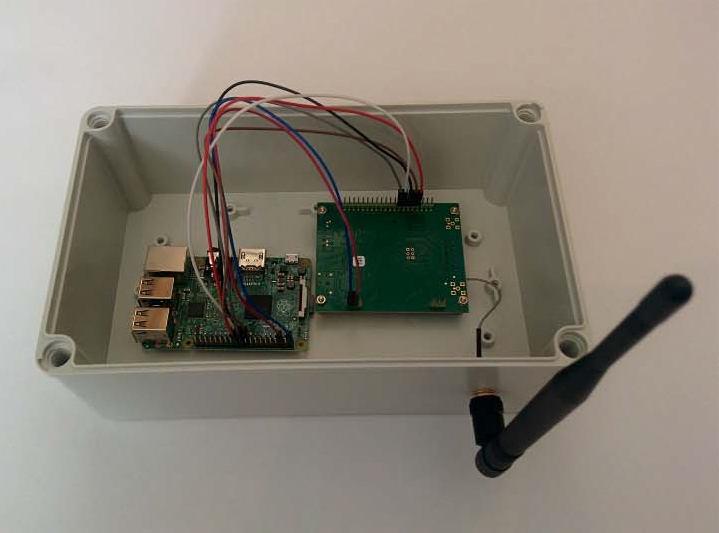
\includegraphics[width=0.6\textwidth]{img/gateway/gateway.jpg}

\newpage
\section{Messungen}
Die vorgängig definierten Routen werden abgelaufen und die Messungen werden an den definierten Standorten durchgeführt.

\section{Auswertung}
Die erhobenen Daten werden analysiert und kategorisiert. Messungen sollen in 3 Kategorien eingeteilt werden.
\begin{enumerate}
	\item Direkter Sichtkontakt
	\item Wenig Sichtkontakt resp. teilweise blockiert. Bspw. durch Bewaldung oder Steinformationen
	\item kein ein Sichtkontakt zwischen Empfänger und Sender.
\end{enumerate}


\subsection{Installation Software}
Die Installation der Gateway Software wird von TTN bereitgestellt und von der Community aktiv verwaltet und verbessert. Die TTN Community Gruppe aus Zürich hat ein sehr simples Installationsskript zusammengestellt um die Gateway Software automatisiert zu installieren.

Vorgehen auf dem Gateway
\begin{enumerate}
	\item Paketdefinitionen geupdated
	
\end{enumerate}
Code:
apt-get update
apt-get upgrade

%sudo dpkg-reconfigure locales // de_CH
sudo dpkg-reconfigure tzdata // Europe/Zurich

sudo raspi-config // Enable SPI

git clone https://github.com/ttn-zh/ic880a-gateway.git ~/ic880a-gateway
cd ~/ic880a-gateway

change EUI Source to Wireless
%GATEWAY_EUI_NIC="wlan0"

sudo ./install.sh spi



\chapter*{Selbständigkeitserklärung}
\label{chap:selbstaendigkeitserklaerung}

\vspace*{10mm} 

Ich bestätige, dass ich die vorliegende Arbeit selbstständig und ohne Benutzung anderer als der im Literaturverzeichnis angegebenen Quellen und Hilfsmittel angefertigt habe. Sämtliche Textstellen, die nicht von mir stammen, sind als Zitate gekennzeichnet und mit dem genauen Hinweis auf ihre Herkunft versehen. 

\vspace{15mm}

\begin{tabbing}
xxxxxxxxxxxxxxxxxxxxxxxxx\=xxxxxxxxxxxxxxxxxxxxxxxxxxxxxx\=xxxxxxxxxxxxxxxxxxxxxxxxxxxxxx\kill
Ort, Datum:\> Bern, 15.01.2018 \\ \\
Namen Vornamen:\> Martin Schmidli  \\ \\ \\ \\ 
Unterschriften:\> ...................................... \\
\end{tabbing}

\chapter*{Anhang}
\section{Software}
Es wird kein Code direkt an dieses Dokument angehängt. Zur Verwaltung des Sourcecodes wurde die Plattform Github verwendet. Jegliche Commits vor dem 16.09.2017 gehören zur Projekt 2 Arbeit. Commits nach diesem Datum wurden im Zuge der Bachelor Thesis erstellt. 
Folgend Sie den Links um den Sourcecode einzusehen.
\subsection{Atas-Webapp}
\url{https://github.com/schmm2/atas-webapp}
\subsection{Atas-Service}
\url{https://github.com/schmm2/atas-service}
\subsection{Atas-Node}
Software welche auf dem 1. Prototypen eingesetzt wird\\
\url{https://github.com/schmm2/atas-node}
\subsection{Atas-Node2}
Software welche auf dem 2. Prototypen eingesetzt wird\\
\url{https://github.com/ATAS-Group/atas-node2}



\printglossaries

\listoffigures

\begin{thebibliography}{1}
	\bibitem{kammerlander} \url{https://www.bergwelten.com/a/die-schoensten-zitate-rund-ums-bergsteigen} 1.2.2018
	\bibitem{sacaccident} \url{http://www.sac-cas.ch/unterwegs/sicherheit/bergnotfallstatistik.html} 1.2.2018
	\bibitem{wavelengthTTN} \url{https://www.thethingsnetwork.org/forum/t/antenna-length-for-868-and-433-mhz/5378} 2.1.2018
	\bibitem{wavelength} \url{https://en.m.wikipedia.org/wiki/Wavelength} 2.1.2018\\
	\bibitem{avalanche} \url{http://www.oegan.at/notfallmedizin/index.php?option=com_content&view=article&id=76:unterkuehlung-als-ueberlebenschance&catid=42&Itemid=118} 1.01.2018
	\bibitem{ttnsecuirty} \url{https://www.thethingsnetwork.org/wiki/LoRaWAN/Security} 27.07.2017
	\bibitem{jaguar} \url{https://www.jaguar-network.com/en/news/lorawan-in-a-nutshell-2-internet-of-things-iot}, 27.07.2017
	\bibitem{ADRTTN} \url{https://www.thethingsnetwork.org/wiki/LoRaWAN/ADR} 27.07.2017
	\bibitem{autodesk} \url{https://www.autodesk.com/products/eagle} 27.07.2017
	\bibitem{espidfarduino} \url{http://iot-bits.com/documentation/esp32-tutorial-and-example-programs/} 20.12.2017
	\bibitem{espidfinstallation} \url{https://dl.espressif.com/doc/esp-idf/latest/get-started/index.html} 27.12.2017
	\bibitem{espidfdriver} \url{https://www.silabs.com/products/development-tools/software/usb-to-uart-bridge-vcp-drivers} 27.12.2017
\end{thebibliography}

\end{document}